\documentclass[9pt,a4paper,fleqn,portrait]{scrartcl}
\usepackage[utf8]{inputenc}
\usepackage[english]{babel}

%--------------------------------Layout ------------------------------------
\usepackage{multicol}	% multiple columns
\usepackage{graphicx}	% images
\usepackage{xcolor}		% color
\usepackage{todonotes}
\usepackage{tabularx,ragged2e}
\usepackage{array, makecell}

%--------------------------------Pseudocode------------------------------------------
\usepackage[linesnumbered, ruled]{algorithm2e}
\SetKwRepeat{Do}{do}{while} 					
\SetKwRepeat{DoUntil}{do}{until}
\SetKwRepeat{RepeatUntil}{repeat}{until}


%% ----- Text -----															
\usepackage[sfdefault]{cabin}	% font
\setlength\parindent{0pt}		% no indent after paragraph

\usepackage{enumitem}			% lists
\setlist{nosep}
\setlist[itemize]{leftmargin=1em}
\setlist[enumerate]{leftmargin=*}


% --------------------------- tikz
\usepackage{environ}
\usepackage{fontawesome}
%\usepackage[tikz]{bclogo}
\usepackage{tikz}
\usetikzlibrary{calc}




%% ----- Geometry -----
\usepackage[
landscape,
left 		= 1.0cm,
right 		= 1.0cm,
top			= 1.0cm,
bottom		= 1.2cm
]{geometry}
\setlength{\footskip}{15pt}
\setlength\columnsep{15pt}


%--------------------------------Math------------------------------------------
\usepackage{amsmath, amsfonts, amssymb, bm, bbm, mathtools, mathrsfs, units, empheq, gensymb}	
\usepackage[makeroom]{cancel}	% cross out math expressions
\usepackage{ dsfont }

%--------------------------------- Hyperlinks --------------------------------------
\PassOptionsToPackage{hyphens}{url}	
\usepackage[pdftex,
		a4paper,
		bookmarks,
		bookmarksopen=true,
		bookmarksnumbered=true,
		pdfauthor={V\'{e}ronique Kaufmann},       
		pdftitle={AML 2020 Summary},   
		colorlinks = true,
		linkcolor=black,
		citecolor=black,
		filecolor=black,
		urlcolor=cyan,
		anchorcolor=black,
		menucolor=black,
		breaklinks=true,
		pageanchor=true,
		plainpages=false,
		pdfpagelabels=true]{hyperref}

\hypersetup{
    colorlinks=true,
    linkcolor=black,
    filecolor=magenta,      
    urlcolor=cyan,
}

%---------------------------------Commands--------------------------------------
% separation line between sections (not used)
\newcommand{\sepline}{\par\centerline{\rule{\columnwidth}{0.4pt}}\par}

% basics
\newcommand{\norm}[1]{\left\lVert#1\right\rVert}
\newcommand{\argmin}{\mathop{\mathrm{argmin}}}
\newcommand{\argmax}{\mathop{\mathrm{argmax}}}
\newcommand{\mean}[1]{\overline{#1}}
\newcommand{\inv}[1]{{#1}^{-1}}
\newcommand{\transp}[1]{{#1}^\top}

% numbers
\newcommand{\R}{\mathbb R}				% real numbers
\newcommand{\N}{\mathbb N}				% natural numbers


% symbols used for probabilities and datasets
\newcommand{\E}{\mathbb E}				% expectation
\renewcommand{\P}{\mathbf P}		% probability
\newcommand{\X}{\mathbf X}		% Matrix containing all input vectors
\newcommand{\x}{\mathbf x}		% input vector
\newcommand{\z}{\mathbf z}		% input vector

\newcommand{\y}{\mathbf y}		% labels
\newcommand{\w}{\mathbf w}		% weight vector


\newcommand{\K}{\mathcal K}				% kernel function
\renewcommand{\L}{\mathcal L}			% loss function

% sums
\newcommand{\sumi}[1]{\sum_{i = 1}^{#1}}
\newcommand{\sumj}[1]{\sum_{j = 1}^{#1}}
\newcommand{\sumin}[0]{\sum_{i\leq n}}
\newcommand{\sumim}[0]{\sum_{i\leq m}}


% Ensemble methods
\newcommand{\bbar}{\mathchar'26\mkern-9mu b}

% Neural Nets
\newcommand{\weight}[1]{w^{(#1)}}		% weight with power index
\newcommand{\activation}[1]{a^{(#1)}}	% activation with power index
\newcommand{\bias}[1]{b^{(#1)}}			% bias with power index
\newcommand{\nnout}[1]{z^{(#1)}}			% output with power index


\newcommand{\ap}[1]{\alpha^{(#1)}}		% activation function with power index
\newcommand{\Lp}[1]{L^{(#1)}}			% linear functions
\newcommand{\NN}{\mathit{NN}}			% neural net
\newcommand{\enc}{\mathit{enc}}			% encoder function (autoencoders)


% Bayesian Methods, Distributions
\newcommand{\Dir}{\mathit{Dir}}			% Dirichlet Distribution
\newcommand{\Beta}{\mathit{Beta}}		% Beta Distribution
\newcommand{\DP}{\mathit{DP}}			% Dirichlet process
\newcommand{\GEM}{\mathit{GEM}}			% GEM distribution


% PAC learning
\newcommand{\RIG}[0]{\hat{\mathcal R}\mathit{IG}}

% -------------------------Colors -----------------------------------------------
\definecolor{imp}{RGB}{127, 0, 255}
\definecolor{imp2}{RGB}{0, 204, 102}
\definecolor{imp3}{RGB}{51, 153, 255}
\definecolor{highlight}{RGB}{189, 255, 228}


% ----------------------- Highlight for important stuff -------------------------
\NewEnviron{highlight}[1]
  {\par\medskip\noindent
  \begin{tikzpicture}
    \node[inner sep=0pt] (box) {\parbox[t]{.99\textwidth}{%
    \noindent\fcolorbox{highlight}{highlight}{
%          \begin{minipage}{.1\columnwidth}
%          \centering\tikz[scale=1]\node[scale=3,rotate=0]{\faExclamation};
%          \end{minipage}%
          \begin{minipage}{\columnwidth}
          \textbf{\textit{#1}}\par\medskip
          \BODY
          \end{minipage}\hfill}%
      }
    };
  \end{tikzpicture}\par\medskip%
}

% Title
\title{Advanced Machine Learning \\ 
			{HS 2020}
		}
\author{V\'{e}ronique Kaufmann}


\begin{document}	

%------------------------------Table of Contents --------------------------------
\begin{multicols*}{4}
	{\footnotesize 
		\tableofcontents
	}
	\listoftodos
	\columnbreak
	
	\section*{References: }
	{\footnotesize
		\textbf{General: }
\begin{itemize}[leftmargin=*]
	\item Advanced Machine Learning Course 2020, ETHZ
	\item Standord CS229 course: \\
		\url{http://cs229.stanford.edu/syllabus-fall2020.html} 
\end{itemize}

\textbf{Ensemble methods: }
\begin{itemize}[leftmargin=*]
	\item Images of Bagging, Boosting, Random Forest: \\
		\url{https://towardsdatascience.com/ensemble-methods-bagging-boosting-and-stacking-c9214a10a205}
\end{itemize}

\textbf{Clustering}
\begin{itemize}[leftmargin=*]
	\item k-means vs EM\\
	\url{https://towardsdatascience.com/a-comparison-between-k-means-clustering-and-expectation-maximization-estimation-for-clustering-8c75a1193eb7}
\end{itemize}
	}
\end{multicols*}	
\newpage	


\begin{multicols*}{3}
	\pagenumbering{arabic}
	\maketitle
	%\section{Introduction}
%\todo[inline]{TODO: Might want to place a summary here..}

\setcounter{section}{1}			
	\section{Representations}
Goal of learning is to minimize the expected classification error, while maximizing generalization (avoid overfitting!).
We can't really do this. But we can minimize the \textit{empirical classification error} and maximize the \textit{estimated empirical generalization performance} by cross validation.

\subsection{The learning Problem}
\begin{itemize}
	\item Find function $f : \mathcal{X} \rightarrow \mathcal{Y}$ 
	\item Loss function $Q$ measures the deviation between $y$ and $f(x)$
	\begin{itemize}
		\item $(y-f(x))^2$ \quad  quadratic loss (regression)
		\item $\mathbb{I}_{\{y\neq f(x)\}}$ \quad 0-1 loss (classification)
		\item $\exp{(-\beta yf(x))}$ \quad  exponential loss (classification)
	\end{itemize}
	\item Conditional expected risk: \\$R(f,X) = \int_\mathcal{Y} Q(Y, f(X))P(Y|X)dY$
	\item Total Expected Risk: 
	\begin{multline*}
		R(f) = \mathbb{E}_X\left[R(f,X)\right]  = \int_\mathcal{X} R(f, X)P(X)dY\\ 
		= \int_\mathcal{Y} \int_\mathcal{X} Q(Y, f(X))P(X, Y)dXdY
	\end{multline*}
\end{itemize}

We divide the data intro training and test data to make sure we don't use the test data for calidation.
\begin{itemize}
	\item Empirical Risk Minimizer $\hat f \in \arg \min \hat R(f, \mathcal{Z}^{\text{train}})$ 
	\item Training Error: $\hat R(\hat f, \mathcal{Z}^\text{train}) = \frac{1}{n}\sum_{i=1}^n Q(Y_i, \hat f(X_i))$ 
	\item Test Error: $\hat R(\hat f, \mathcal{Z}^\text{test}) = \frac{1}{m}\sum_{i=n+1}^{n+m} Q(Y_i, \hat f(X_i))$
\end{itemize}

\subsubsection{Typical Approach}
\begin{enumerate}
	\item Feature Extraction (transform raw data to reduce information)
	\item Classifier Design
	\item Post-processing of classification results (adapt classifier output to enable stable scoring)
	\item Scoring
\end{enumerate}

\subsection{Taxonomy of Data}
Pattern Analysis = Find structure in sets of object representations.

\begin{itemize}
	\item Object Space $\mathcal{O}$
	\item Measurement mapping $x$ into a domain $\mathbb{K}$
\end{itemize}

\subsubsection{Data}
\begin{itemize}
	\item Monadic data: $X \to \mathbb R^d, o\mapsto X_o$ (water depth, temperature, pressure, intensity, ...)
	\item dyadic data $\mathcal O^{(1)} \times \mathcal O^{(1)} \to \mathbb R, (o_1, o_2) \mapsto X_{o_1, o_2}$ (e.g. (Users, Websites)). \\
		Pairwise Data: $\mathcal O \times \mathcal O \to \mathbb R, (o_1, o_2) \mapsto X_{o_1, o_2}$ (e.g. image patches x image patches)
	\item polyadic data
	\item ...
\end{itemize}
\begin{center}
	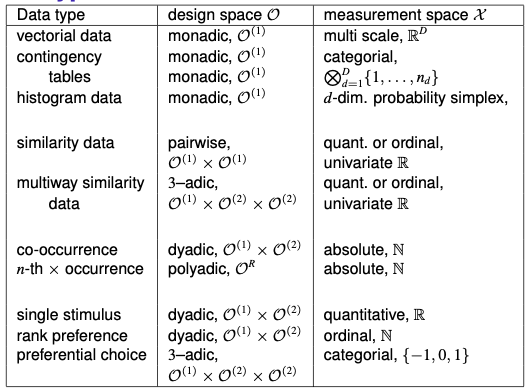
\includegraphics[width=0.8\columnwidth]{images/2-datatypes}
\end{center}

\subsection{Scales}
\begin{itemize}
	\item Nominal / Categorical: qualitattive, but without quantitative measurements (e.g. categories, binary, ...)
	\item Ordinal Scale: Values only meaningful w.r.t other measurements (rank order carries information, not the numerical differences)
	\item Quantitative Scale:
	\begin{itemize}
		\item Interval scale: relation of numerical differences carries the information
		\item Ratio scale: zero value of the scale carries information, but not the measurement unit
		\item Absolute scale: Absolute value is meaningful
	\end{itemize}
\end{itemize}

\subsection{Learning Pipeline: }
\begin{center}
	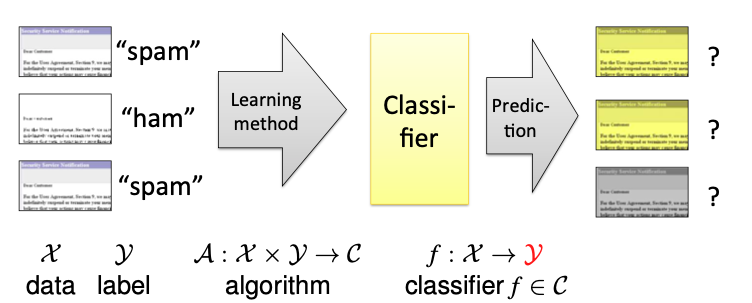
\includegraphics[width = 0.8\columnwidth]{images/2-pipeline}
\end{center}

\subsection{Mathematical Spaces}
A pair of objects $(\mathcal X, d)$ consisting of a non-empty set $\mathcal X$ and a function $d:\mathcal X \times \mathcal X \to \mathbb R$ is called a \textbf{metric space}, if:
\begin{enumerate}
	\item Positivity: $d(x,y) \geq 0 \forall x,y \in \mathcal X$
	\item Uniqueness $d(x,y) = 0 \iff x = y$
	\item Symmetry $d(x,y) = d(y,x)$
	\item $\triangle$-inequality: $d(x,z) \leq d(x,y) + d(y,z), x,y,z\in \mathcal X$
\end{enumerate}

\subsubsection{Euclidean Vector Space}
Let $\mathcal V = (\mathcal X, +, \cdot)$ a vector space. $x,y \in \mathcal V$. $\phi:\mathcal X \times \mathcal X \to \mathbb R$ is called \textbf{scalar product} if:
\begin{enumerate}
	\item Distributivity: $\phi(x_1. + x_2, y) = \phi(x_1, y) + \phi(x_2, y)$
	\item Commutativity: $\phi(x,y) = \phi(y,x)$
	\item Homogeneity: $\phi(\alpha x, y) = \alpha\phi(x,y)$
	\item Positive Definiteness: $\phi(x,x) > 0 \quad \forall x \neq 0$
\end{enumerate} 
A vector space with a scalar product is called \textbf{euclidean vector space}.

\subsubsection{Probability Spaces}
\begin{itemize}
	\item Elementary event: $\omega_1, ...k, \omega_N$ are sample points
	\item Sample space: $\Omega = \{\omega_1, ..., \omega_N\}$
	\item Family of Sets: Event $A$ of an experiment is a set of elementary events with $A \subset \Omega$, result of experiment is $\omega \in A$ or $\omega \not\in A$
	\item Algebra of events $\mathcal A$ = set of subsets $A\subset \Omega$ with $\Omega \in \mathcal A$ and $(A\in \mathcal A \land B \in \mathcal A \implies A\cup B \in \mathcal A \land A \cap B\in \mathcal A \land A \backslash B \in \mathcal A)$
\end{itemize}
Assign weights to elementary events with $0\leq p(\omega_i) \leq 1$ and $\sum_ip(w_i) = 1$. The \textbf{Probability of an event} $A\in \mathcal A$ with $P(A) = \sum_{\{i:w_i\in A\}} p(w_i)$

A \textbf{probability model} is a triple $(\Omega, \mathcal A, P)$, with $\mathcal P = \{P(A) \mid A \in \mathcal A\}$

\sepline 		
	\section{Density Estimation with Parametric Models}
\subsection*{Overview: }
\begin{itemize}
	\item Maximum Likelihood estimation \\
	$$\theta_{MLE} = \arg\max p(X\mid\theta) = \arg \max \sum_i p(x_i\mid\theta)$$
	\item Maximum a Posteriori estimation \\
	\begin{multline*}	
	\theta_{MAP} = \arg\max P(\theta\mid X) = \arg\max P(X\mid\theta)p(\theta) \\
	= \arg \max \sum_i(\log{p(x_i\mid \theta)} + \log p(\theta))
	\end{multline*}
	\item If we have uniform distribution in the prior, the last term of the MAP sum goes away and we have $\theta_{MAP} = \theta_{MLE}$.
\end{itemize}

\subsection{Bayesianism: MAP estimation}
Assume $p(x)$ is unknown, $p(x\mid \theta)$ is known. We want to copmute $p(X=x \mid \mathcal X)$
\begin{itemize}
	\item Prior P(model)
	\item likelihood P(data $\mid$ model)
	\item Posterior: P(model $\mid$ data)
	\item evidence: P(data)
	\item Bayes Rule: 
	$$P(model \mid data) = \frac{P(data\mid model)P(model)}{P(data)}$$
\end{itemize}

\subsection{Frequentism (Fisher): ML estimation}
\begin{enumerate}
	\item Define parametric model (e.g. $\mathcal N(\theta, 1)$)
	\item Define the likelihood as a function of the parametric model (probability of the observations given the parameter $\theta$), e.g.
	$$
		\mathbf P(y_1, ..., y_n \mid \theta) = \prod_{i\leq n}\mathbf P(y_i\mid \theta) = \prod_{i\leq n}\mathcal N(y_i, \theta, 1)
	$$
	\item compute an estimator by maximizing the likehood $\hat\theta_{ML} = \arg\max_\theta \mathbf P(y_1, ..., y_n \mid \theta)$, usually using the log-likelihood.
\end{enumerate}

\textbf{Properties of ML Estimators:}
\begin{itemize}
	\item Consistent ($\theta_{ML} \to \theta_0$) as $n\to \infty$
	\item Asymptotically normal: $1/\sqrt n (\theta_{ML} - \theta_0)$ converges in distribution to a random variable with distribution $\mathcal N(0, J^{-1}(\theta)I(\theta)J^{-1}(\theta)$
	\item Asymptotically efficient: $\theta_{ML}$ minimizes $\mathbb E\left[(\theta_{ML} - \theta_0)^2\right]$. I.e. $\mathbb E\left[(\theta_{ML} - \theta_0)^2\right] = \frac{1}{I_n(\theta_0)}$ (See Rao-Cramer Bound)
\end{itemize}

\subsubsection{Rao Cramer Bound}
There exists no estimator such that $\mathbb E\left[(\hat\theta^* - \theta_0)^2\right] = 0$, 
	$$
		\mathbb E\left[(\hat\theta - \theta_0)^2\right] \geq \frac{1}{I_n(\theta_0)} \text{ for any unbiased estimator $\hat\theta$ of $\theta_0$}.
	$$
	where $I_n(\theta_0)$ is the Fisher Information: $$I_n(\theta_0) = n\mathbb V_{\theta_0}\left[\left[
								\frac{\partial}{\partial\theta} \log \mathbf P(Y \mid \theta)
						\right]_{\theta_0}\right]$$

\subsubsection{Stein estimator}
For finite samples, the ML estimator is not necessarily efficient.
$$
	\hat\theta_{JS} = \left(1 - \frac{(d-2)\sigma^2}{\norm{y}^2}\right) \mathbf y
$$

is better for a multivariate random variable with distribution $\mathcal N(\theta_0, \sigma^2 I)$ with range $\mathbb R^d, d\geq 3$.

\subsection{Conclusion}
\begin{center}
	\begin{tabular}{ p{0.47\columnwidth} | p{0.45\columnwidth} } 
		\textbf{Bayesian Method} & \textbf{Frequentist method}\\\hline
		Allows priors & Does not allow priods \\\hline
		Provides distribution when estimating parameters & Provides a single-point when estimating parameters \\\hline
		Requires efficient integration methods (when computing posteriors) & Only requires differentiation methods when estimating parameters \\\hline
		The prior often induces a regularization term &  consistent, equivariant, asympt. normal + efficient \\
	\end{tabular}
\end{center}

\subsection{Summary ML Estimators}
\begin{itemize}
	\item Bias of an estimator: $\mathbf{bias}(\hat\theta_n) = \E[\hat\theta_n] - \theta$: deviation from the true parameter
	\item consistent estimator: $\forall\epsilon > 0, \mathbb P\{|\hat\theta_n - \theta| > \epsilon\} \xrightarrow{n\to \infty} 0$
	\item Efficiency: ML estimators are \textbf{asymptotically efficient}: 
	$$
		\lim_{n\to\infty}\left(\mathbb V[\hat\theta^{ML}(x_1, ..., x_n)]I(\theta)\right)^{-1} = 1
	$$
	$$ I(\theta) = \mathbb V\left[\frac{\partial\log P(x_1, ..., x_n|\theta)}{\partial \theta} \right]$$
	\item 
\end{itemize}

\subsection{ML vs. Bayes Estimation (MAP)}
\begin{itemize}
	\item They are asymptotically equivalent
	\item Advantage of ML: Only need differential calculus and gradient descent techniques. Bayes needs integration.
	\item A "flat" prior yields little information, since the model uncertainty is not significantly reduced.
\end{itemize}




	
	\section{Regression}
\begin{itemize}
	\item Optimal solution for regression $\arg\min_f\E(Y - f(X))^2$ given by $f^*(x) = \E(Y \mid X=x)$ \\
		However, $\P(Y\mid X)$ and $\P(X)$ are unknown
	\item \textbf{(Parametric) maximum likelihood: }
	\begin{enumerate}
		\item Assume $Y\mid X \sim \mathcal N(f(X), \sigma^2\mathbf I)$
		\item Solve $\arg\max_f\sum_{i = 1}^n \log\P(Y = y_i\mid X=x_i, \sigma^2)$
	\end{enumerate}
	\item \textbf{Statistical learning theory: } \\ Directly minimize empirical risk $\arg\min_f\sum_{i = 1}^n (y_i - f(x_i))^2$
\end{itemize}
\subsection{Linear Regression}
$$
	Y = \beta_0 + \sum_{j = 1}^d X_j\beta_j = X^T\beta, Y\in \mathbb R
$$
\text{$\beta_0$ is called bias, $X,\beta \in \mathbb R^{d+1}$.}


Ordinary least squares regression model: least-squares cost function. 
\begin{itemize}
	\item[$\Rightarrow$] Minimization either through gradient descent or closed form solution 
\end{itemize}
\subsubsection{Residual Sum of Squares (RSS)}

$
	RSS(\beta) = \sum_{i = 1}^n (y_i - x_i^T\beta) = (\mathbf y - \mathbf X\beta)^T(\mathbf y - \mathbf X\beta)
$

$\nabla_\beta RSS(\beta) = 0 \implies \hat\beta = (\mathbf{X^TX})^{-1}\mathbf X^T\mathbf y$


\subsubsection{Prediction}
$$
	\hat{\mathbf y} = \mathbf X \hat\beta = \mathbf X(\mathbf X^T\mathbf X)^{-1}\mathbf X^T \mathbf y, 
$$
where $\mathbf X(\mathbf X^T\mathbf X)^{-1}\mathbf X^T$ is an orthogonal projectin on the space spanned by the columns of $\mathbf X$.

\begin{itemize}
	\item Assume additive gaussian noise: $Y = \beta_0 + \sum_{j = 1}^d X_j\beta_j + \epsilon = X^T\beta + \epsilon $ with conditional mean $\E(Y\mid X_1, ..., x_d) = X^T\beta$
	\item Distribution: $\hat \beta \sim \mathcal N(\beta, (\mathbf X^T\mathbf X)^{-1}\sigma^2)$
\end{itemize}

\subsubsection{Local weighting}
We can add weights to the features, such that not all of them are treated equally:
\begin{equation*}
	\hat\beta = \argmin_\beta \sum_i w_i (y_i - \transp{x_i}\beta)^2 
\end{equation*}

If $w_i$ is large, this feature will become very important, if $w_i$ is small it will be pretty much ignored.

Predict: $y = x\beta$


\subsection{Bias / Variance Dilemma}
Goal: Minimize bias and variance simultaneously (usually impossible).
\begin{itemize}
	\item Data $D = \{(x_i, y_i)_{i = 1}^n\}, y_i\in \mathbb R$
	\item Objective: Find regression function $f\in \mathcal C$ such that $\E( Y - f(X))^2$ is minimal.
	\item Optimum $f^*(x) = \E(Y \mid X=x)$
	\item Estimator $\hat f(X)$ depends on random variable $X$ and data $\mathcal D$
	\item \textbf{Problems: } we only have a finite training set, and the complexity of hypothesis class $\mathcal C$ is unknown.
\end{itemize}

\vspace{1em}
\textbf{Tradeoff: }
\begin{itemize}
	\item Small data sets and large $\mathcal C$: Variance large, bias small
	\item Large data set, small $\mathcal C$: Variance small, bias large
\end{itemize}
\textit{The optimal tradeoff between bias and variance is achieved when we avoid both underfitting (large bias) and overfitting (large variance)}

\vspace{1em}
\textbf{Prediction error: }
\begin{align*}
		\E_D\E_{Y\mid X=x}\left(\hat f(x) - Y\right)^2 &=\\
	(\text{variance})\quad &\E_D(\hat f(x) - \E_D(\hat f(x))^2 \\
	(\text{bias$^2$})\quad &+ \left(\E_D(\hat f(x)) - \E(Y\mid X=x)\right)^2 \\
	(\text{noise})\quad &+  \E(Y - \E(Y\mid X=x))^2
\end{align*}

\subsection{Overfitting}
\begin{itemize}
	\item \textbf{Regularization}: Add model complexity term to cost function 
	$\arg\min_\theta\sumi n l(f(x_i, \theta, y_i) + R(\theta) $\\
	Often equivalent to choosing a prior in a bayesian framework and using a MAP estimator.
	\item Model selection based on \textbf{generalization error estimate} (e.g. cross-validation)
	\item \textbf{Ensembles} of classifiers (See Section 9)
\end{itemize}



\subsection{Ridge Regression, LASSO}
\begin{center}
{\footnotesize
	\begin{tabular}{ p{0.1\columnwidth} | p{0.39\columnwidth} | p{0.39\columnwidth} } 
		& \textbf{Ridge Regression} & \textbf{LASSO}\\\hline
			
		Reg. $R$ & $\lambda\beta^T\beta$ & $\lambda\norm{\beta}_1$ \\\hline
		Bay. view: & $Y | (X, \beta) \sim$ $\mathcal N(x^T\beta, \sigma^2\mathbf I)$, 
		
		prior $\beta: \beta\sim\mathcal N(0, \sigma^2 / \lambda\mathbb I)$ & 
			$Y | (X, \beta) \sim$ $\mathcal N(x^T\beta, \sigma^2\mathbf I)$, Laplace prior:
			
			 $p(\beta_i) = \frac{\lambda}{4\sigma^2}\exp(-|\beta|\frac{\lambda}{2\sigma^2})$
		\\\hline
		Solution & $\hat\beta_\lambda^{\textit{ridge}} = (\mathbf X^T\mathbf X + \lambda\mathbf I)^{-1}\mathbf X^T\mathbf y$ & Optimization techniques 
		
			(e.g. LARS), $\norm{\beta}_1$ is not differentiable. \\\hline
	\end{tabular}
	}
\end{center}

\subsubsection{Singular Value Decomposition}
\begin{itemize}
	\item Take centered $X$ and perform SVD: $X = UDV^T$ ($U, V$ have orthonormal columns)
	\item SVD of least squares fitted vector: 
	
	$\X\hat\beta^{ls} = \X(\X^T\X)^{-1}\X^T\y = \mathbf U \mathbf U^T\y$
\end{itemize}

\subsubsection{Ridge regression: }
If the $\beta_j$ are unconstrained, they can explode (high variance). We can \textbf{control the variance by regularizing the coefficients: }

\vspace{1em}
\textbf{Constraint: }
\begin{align*}
	&\min \sumi n(y_i - \transp{\beta}x_i)^2 \textit{ s.t. } \sumj d \beta_j^2 \leq t \\
	\iff &\min \transp{(y- \X\beta)}(y-\X\beta)  \textit{ s.t. } \sumj d \beta_j^2 \leq t \\
	&\textit{Assume $\X$ standardized, $\y$  centered}
\end{align*}
We can rewrite this as
\begin{align*}
	\mathit{PRSS}(\beta)_{l_2} 	&= \sumi n(y_i - \transp{x_i}\beta)^2 + \lambda\sumj d \beta_j^2 \\
								&= (\y - \X\beta)^\top(\y - \X\beta) + \lambda\norm{\beta}^2
\end{align*}

\begin{align*}
	\X\hat\beta^{\text{ridge}} &= \X(\X^T\X + \lambda\mathbf I)^{-1}\X^T\y \\
	&= \mathbf{UD} (\mathbf D^2 + \lambda \mathbf I)^{-1}\mathbf{DU}^T\y \\
	&= \sumi d \mathbf u_j  \frac{d_{j}^2}{d_{j}^2 + \lambda} \mathbf u_{j}^T\mathbf y 
\end{align*}



$\frac{d_j^2}{d_j^2 + \lambda}$ is small for small singular values $d_j$ and goes to 1 for large SV. This suppresses contributions of small eigenvalues.
\begin{itemize}
	\item $\hat \beta^\textit{ls} = \beta + (\textit{Inflammation term dep. on $\inv{\Sigma}$}) \epsilon$ (\href{https://kunyu-he.com/2020/01/11/SVD-in-Machine-Learning-Ridge-Regression-and-Multicollinearity/}{Derivation})
	\item With multicollinearity (i.e. columns of $\X$ are not independent), some $d_i, d_j$ will be close to 0. The diagonal element $1/d_j$ will then be huge. 
	\item This leads to large inflammation term and therefore \textbf{great deviation in the least squares weights from the true weights.}
	\item Ridge regression projects $\y$ onto the components with large $d_j$
	\item This shrinks the coefficients of low-variance components.
\end{itemize}

\subsubsection{The LASSO (Least Absolute Shrinkage and Selection Operator)}
\begin{align*}
	\hat\beta^{\text{LASSO}}  	&= \argmin_\beta \sumi n(y_i- \beta_0 - \sumj d x_{i,j}\beta_j)^2 \\
								&= \argmin_\beta (\y - \X\beta)^\top(\y-\X\beta)\\
	&\text{subject to} \sumj d|\beta_j| \leq s.
\end{align*}

We can rewrite this as
\begin{align*}
	\mathit{PRSS}(\beta)_{l_1} 	&= \sumi n(y_i - \transp{x_i}\beta)^2 + \lambda\sumj d |\beta_j| \\
								&= (\y - \X\beta)^\top(\y - \X\beta) + \lambda|\beta_j|
\end{align*}

\textit{LASSO estimates are known to be sparse with few coefficients non-vanishing (Reason: LSE error surface hits the corners of the constraint surface often).
}
\begin{center}
	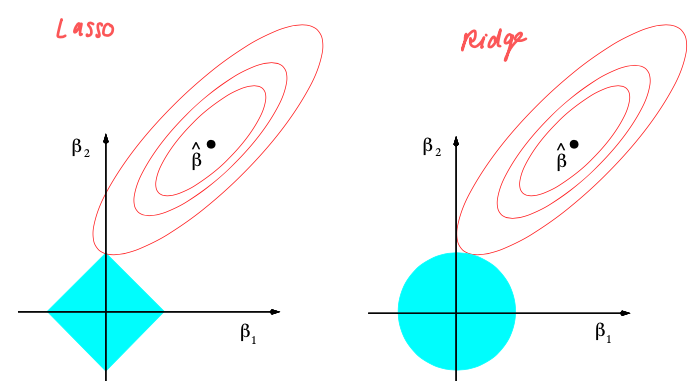
\includegraphics[width=0.8\columnwidth]{images/4-ridge-vs-lasso}\\
	\textit{Contours of error and constraint functions. Blue = constraint regions, red=contours of least squares error function.}
\end{center}
\begin{itemize}
	\item Often, we believe that some $\beta_j$ should be $0$.
	\item Large $\lambda$ will set some coefficients equal to $0$ $\to$ sparse solution
	\item \textbf{LASSO will perform model selection for us}
\end{itemize}


\subsection{nonlinear regression with basis expansion}
\textbf{Idea: } Transform variables $X$ nonlinearly and fit a linear model in the resulting feature space.

\begin{equation*}
	\begin{gathered}			
		f(X) = \sum_{m=1}^M \beta_mh_m(X) \\
		h_m(X) : \R^d\mapsto \R, 1\leq m \leq M
	\end{gathered}
\end{equation*}

\textbf{Smoothing Splines:}	
Cubic splines are a common choice for $h$.
\begin{itemize}
	\item Know selection: Use the maximal number of knots and control the smoothness by regularization:
	$$
		RSS(f, \lambda) = \sumi n(y_i - f(x_i))^2 + \lambda\int(f''(x))^2 dx
	$$
\end{itemize}

\subsection{Regression with Wavelets}
Many phenomena are local perturbations (e.g. face muscles) and can hence be modeled by wavelets (?).

Haar wavelet, symmlet-8 wavelet, denoising by wavelet shrinkage
			
	\section{Gaussian Processes}
Different way to go nonlinear.

Remember linear regression: $Y = X^T\beta + \epsilon, \epsilon\sim \mathcal N(\epsilon, 0, \sigma^2)$
or equivalently:
$$
	p(Y\mid X,\beta,\sigma) = \mathcal N(Y\mid X^T\beta, \sigma^2) \propto \exp\left(-\frac{1}{2\sigma^2}(Y - X^T\beta)^2\right)
$$

\subsection{Multivariate Gaussians}
A vector $x\in\R^d$ has multivariate normal distribution with mean $\mu\in\R^d$ and covariance $\Sigma\in \mathbf S^d$ (symmetric positive definite $n\times d$ matrix) $x\sim \mathcal N(\mu, \Sigma)$, if

$$
	p(x;\mu,\Sigma) = \frac{1}{(2\pi)^{d/2}|\Sigma|^{1/2}}\exp\left(-\frac
	1 2 (x-\mu)^T\Sigma^{-1}(x-\mu)\right)
$$

\subsubsection{Why Gaussians are useful}
\begin{itemize}
	\item Common when modeling noise in statistical algorithms (can be considered as accumulation of small independent random perturbations);\\ 
		Summation of independent random variables tend to look gaussian.
	\item Convenient for many analytical manipulations, because many of the integrals that arise have closed form solutions.
\end{itemize}


\subsection{Bayesian Linear Regression} 
\textit{Assume a prior distribution over parameters and obtain posterior using Bayes's rule.}

\vspace{1em}
We can turn conventional multiple linear regression model into a bayesian regression model by defining a \textbf{prior} over the regression coefficients.

\textbf{Goal: } Probabilistic approach; find a distribution over the parameters that gets updated whenever new data points are observed.

$$
	p(\beta\mid\Lambda) = \mathcal N_d(\beta\mid\mathbf 0, \Lambda^{-1})\propto \exp(-1/2 \beta^T\Lambda\beta),
$$
where $\Lambda = \inv \Sigma$ is the precision matrix.

This favors $\beta$ to be $0$. 

The \textbf{Posterior} then becomes:
\begin{align*}
	p(\beta\mid \X, \y, \Lambda) &= \mathcal{N} (\beta\mid\mu_\beta, \Sigma_{\beta})\\
							\mu_\beta	&= (\X^T \X + \sigma^2\Lambda)^{-1}\X^T \y \\
							\Sigma_\beta &= \sigma^2(\X^T \X + \sigma^2\Lambda)^{-1}
\end{align*}

Bayesian linear regression with gaussian prior over the coefficients is equivalent to ridge regression for $\Lambda =\lambda \mathbb I_d, \sigma=1$

\subsection{Gaussian Processes}

\textit{Gaussian processes are the extension of multivariate Gaussians to infinite-sized collections of real-values variables (Gaussian processes are distributions over random functions and not just random vectors).}

\vspace{1em}
\textbf{Goal: } Non-parametric approach: Find a distribution over the possible functions $f(x)$ that are consistent with the observed data (is also a Bayesian approach: Start with a prior, update it whenever new data points are observed; produce posterior).
\begin{itemize}
	\item Moments of joint Gaussian:\\
	 $\E[\y] = \mathbf 0, Cov[\y] = \X\Lambda^{-1}\X^T + \sigma^2\mathbb{I}_n$
	\item Consider the joint distribution over all $\y$:

	$$
		\begin{bmatrix}
			y_1 \\ \vdots \\ y_n
		\end{bmatrix}
			\sim \mathcal N \left(
		\y
		\middle\vert
		\mathbf 0,
			\begin{bmatrix}
				k_{1,1} + \sigma^2 & k_{1,2} & \hdots & k_{1.n} \\
				k_{2,1} & k_{2,2} + \sigma^2 & \hdots & k_{2,n} \\
				\vdots & \vdots & \ddots  & \vdots \\
				k_{n,1} & k_{n,2} & \hdots & k_{n,n} + \sigma^2
			\end{bmatrix}
		\right)
	$$
	where $k_{i,j} = k(x_i, x_j) ) x_i^T\Lambda^{-1} x_j$ is a Kernel function (here, any kernel function could be used, which gives it power and flexibility).
	\item This means, that outputs of points whose inputs are similar to each other, have a high covariance (non-axis-sligned ellipse level set of joint distributions)
\end{itemize}

\subsubsection{Kernel Functions}
Kernel functions specify the degree of similarity between any 2 datapoints. They encode our assumptions about the function we wish to learn (different kernels can obtain very different models).

\textbf{Properties: }
\begin{enumerate}
	\item Symmetry: $k(x,x') = k(x', x)$
	\item Positive Semi-Definiteness: \\
		$k(x,x')f(x)f(x') dxdx' \geq 0 \forall f\in L-2, \Omega\subset \R^d$
\end{enumerate}

The \textbf{Gram Matrix} $\mathbf K$ is positive semi-definite $/iff x^T\mathbf K x\geq 0$


\textbf{Examples of kernel functions: }
\begin{itemize}
	\item Linear kernel: $k(x,x') = x^Tx'$
	\item Polynomial Kernel $k(x,x') = (x^Tx' + 1)^p$
	\item Gaussian (RBF) kernel: $k(x,x') = \exp(-\norm{x-x'}_2^2(h^2)$ (judges how different $x$ and $x'$ are.
	\item Sigmoid (tanh) kernel: $k(x,x') = \tanh \kappa x^Tx' - b$
\end{itemize}

Different kernels have different invariance properties (e.g. invariance to rotation or translation)

\subsubsection{Prediction by Gaussian Processes}
The predictive density $p(y_{n+1} \mid x_{n+1}, \X, \y)$ can be obtained analytically. 

\begin{align*}
		p\left(
		\begin{bmatrix}
			\y \\ y_{n+1}	 
		\end{bmatrix}
		\middle\vert
		x_{n+1}, \X, \sigma
	\right)
	&= \mathcal N
	\left(
		\begin{bmatrix}
			\y \\ 
			y_{n+1}	 
		\end{bmatrix}	
		\middle\vert
		\mathbf 0,
		\begin{bmatrix}
			\mathbf C_n & \mathbf k \\
			\mathbf k^T & c
		\end{bmatrix}
	\right) \\
	\mathbf C_n &= \mathbf K + \sigma^2\mathbf I \\
	c &= k(x_{n + 1}, x_{n+1}) + \sigma^2 \\
	\mathbf k &= k(x_{n+1}, \X) \\
	\mathbf K &= k(\X, \X)
\end{align*}

\begin{algorithm}[H]
	\SetKwInOut{Require}{Require}
	\Require{	\\
				$n$ observed data $\X = (x_1, ..., x_n)^\top \in \R^{n\times d}$, \\
				$k$ kernel function \\
				$\sigma^2$ noise variance
				$x_{n+1}\in\R^d$ new data point 				
				}
				\vspace{1em}
	$\mathbf K \gets (k(x_i, x_j))_{1\leq i,j \leq n}$	{\scriptsize \tcp*[r]{Compute kernel matrix}} 
	$\mathbf k \gets (k(x_{n+1}, x_i))_{1\leq i\leq n}$ {\scriptsize \tcp*[r]{Similarity of new and observed data}}
	$\mu_{y_{n+1}} \geq \transp{\mathbf k}(\mathbf K + \sigma^2\mathbf I)^{-1}\y$ {\scriptsize \tcp*[r]{Mean of predictive distribution}}
	$\sigma^2_{y_{n+1}} \geq k(x_{n+1}, x_{n + 1}) - \transp{\mathbf k}(\mathbf K + \sigma^2\mathbf I)^{-1}\mathbf k$  {\scriptsize \tcp*[r]{Var of  \\ predictive distribution}}
	\vspace{1em}
	\Return{$\mathcal N(y_{n +1}|\mu_{y_{n+1}}, \sigma^2_{n+1})$} {\scriptsize \tcp*[r]{Return predictive distribution}}
	\caption{Prediction with Gaussian processes}	
\end{algorithm}


\subsubsection{Reasons to use Gaussian processes for Regression}
\begin{enumerate}
	\item Like Bayesian methods, GP models allow to quantify uncertainty from errors in the parameter estimation procedure (not just instrinsic noise).
	\item Non-parametric and can hence model essentially arbitrary functions of the input points
	\item Natural ways to introduce kernels into a regressino modeling framework
	\item Simple and straightforward linear algebra implementations
\end{enumerate}

\subsubsection{Wisdom of Crowds}
Averaging over multiple estimators:
\begin{itemize}
	\item unbiased estimators remain unbiased after averaging
	\item Variance is reduced
\end{itemize}


	
	
	
	
	
	
	
		 
	\section{Linear Discriminant Methods}
\textbf{Discriminant methods} aim at estimating $P(X|Y)$ and $P(Y)$ and then use the bayes rule to estimate $P(Y|X)$, instead of directly estimating the latter.
\begin{itemize}
	\item Tend to model a decision boundary between classes / labels. Goal is to find the boundary separating one class from abother
\end{itemize}



\subsection{Discriminative / Generative Models}
Discriminative models model the decision boundary between the classes, while generative model explicitly model the distribution of each class. Reference: \href{https://medium.com/@mlengineer/generative-and-discriminative-models-af5637a66a3}{Medium Blogpost}. 
\subsubsection{Models}
\textbf{Generative model: }statistical model of the joint probability distribution $p(x, y)$ 	\textbf{Important: } Lecture's notation: $p(x, y\mid \theta)$ ,where $\theta$ is the assumed model. \\
	Examples: Hidden Markov Models,  Naive Bayes, Bayesian Networks, LDA/QDA
	
\vspace{1em}
 \textbf{Discriminative model: } Model of the conditional distribution $p(y|x)$ 
		Examples: Threshold functions (perceptron), Fisher's linear discriminant, SVMs, Traditional Neural Networks

\subsubsection{Classifiers}
\textbf{Probabilistic Generative Classifier}\\
\textit{Based on the generative model. Called generative because the joint probability distribution P(X, Y) can be used to generate samples.}
\begin{enumerate}
	\item Assume distribution of labels $(Y|\theta)$
	\item Assume distribution of samples conditioned on labels: $P(X|Y=y)$
	\item Perform MLE over likelihood 
	\begin{equation*}
		P(\X, \y|\theta) = P(\y)P(\X|\y, \theta)
	\end{equation*}
	\item Compute posterior $P(Y|X)$ with LDA or QDA
	\item Create classifier from $P(y|X)$ using Bayes decision theory
	\begin{equation*}
		y = \argmax_y P(y|X) = \argmax_y P(y)\prod_{i=1}^n p(x_i|y)
	\end{equation*}
\end{enumerate}

\vspace{1em}
\textbf{Probabilistic Discriminative Classifier} \\
\textit{Based on the discriminative models. Called discriminative because classifier can be used to discriminate the value of the target variable $Y$.}
\begin{enumerate}
	\item Assume the posterior has the form $P(Y|X) = \sigma(\transp w x + w_0)$. After normalization $P(Y|X) = \sigma(\transp{\tilde w}x)$
	\item Use MLE over  likelihood 
	\begin{equation*}
		P(\y|\w, \X) = P(\y|\X, \w)
	\end{equation*}
	to get
	\begin{multline*}
		L(w) = \log P(\y|\w, \X)\\
		 = c + \sumin\left[y_i\log\sigma(\transp{\w}) x_i+ (1-y_i)\log(1-\sigma(\transp{\w}x_i) \right]
	\end{multline*}
	\item Do gradient Descent or Newton's method over $\mathit{NL}(w) = -L(w)$, since $L(w)$ is intractable.
	\item Use weight vector $w^*$ to predict.
\end{enumerate}

\vspace{1em}
\textbf{Discriminative Classifier}
\textit{The discriminative classifier is not based on any model, but classifies directly.}
\begin{enumerate}
	\item  Choose a loss function $\L : \mathcal Y \times \mathcal Y \to \R^+$
	\item Approximate expected risk $\E_{X,Y}[\L(y, c(X))]$ with the empirical loss $\hat R = \frac{1}{n}\sumin \L(y_i, c(x_i))$ \textit{(abuse of notation)}
	\item Find the optimal classifier $c^*$, such that $c^* = \argmin_c \hat R$
\end{enumerate}


% =================================== Marginal Distributions ====================================
\subsection{Marginal Distributions Recap}
From $P(X,Y)$, we can compute
\begin{align*}
	P(X) &= \sum_y P(X, Y=y) \\
	P(Y) &= \int_x P(Y, X=x) \\
	P(X|Y) &= P(X,Y)/P(Y) \\
	P(Y|X) &= P(X,Y)/P(X)
\end{align*}



% =================================== Discriminant Functions ====================================
\subsection{Discriminant Functions}
Function that takes an input vector $x$ and assigns it to one of the $k$ classes $\mathcal C_k$

\subsubsection{Least Squares (LDA, QDA)}
Make the model predictions as close as possible to a set of target values.
\begin{itemize}
	\item \textbf{Linear Discriminant Analysis (LDA):} Assume the classes have the same covariances (i.e. $\Sigma_0 = \Sigma_1$)\\ $p(y\mid x) = \sigma(\mathbf w^Tx + w_0)$
	\item \textbf{Quadratic discriminant Analysis (QDA):} General (no cov. assumption) \\
	$p(y\mid x) = \sigma(x^T\mathbf Wx + x^T\mathbf w + w_0)$ 

\end{itemize}



\subsubsection{Fisher's Linear Discriminant}
Classification as dimensionality reduction. Goal is to maximize class separation in the output space.

\begin{itemize}
	\item choose $\mathbf w$ to maximize $m_2 - m_1 = \mathbf w^T(\mathbf m_2 - \mathbf m_1)$ with $m_k = \mathbf w^T\mathbf w_k$ ($\mathbf m_i$ is the mean of class $i$).
	
	$$
		w^* \propto S_w^{-1}(\mean{x}_0 - \mean{x}_1)
	$$
	\item Within-class variance: $s_k^2 = \sum_{n\in \mathcal C_k}\mathbf (w^T(x_n - \mean{x}_k))^2$
	\item \textbf{Fisher criterion: } between class variance vs within-class variance: 
	$$
		J(\mathbf w) = \frac{\mathbf w^T(\mean{x}_1 - \mean{x_2})(\mean{x}_1 - \mean{x_2})^T\mathbf w}{s_1^2 + s_2^2} = \frac{\mathbf w^T\mathbf S_B \mathbf w}{\mathbf w^T\mathbf S_W \mathbf w }
	$$,
	where $\mathbf S_B$ is the between-class variance and $\mathbf S_W$ is the within class variance.
	\begin{align*}
		\mathbf S_B &= (\mathbf m_2 - \mathbf m_1)(\mathbf m_2 - \mathbf m_1)^T \\
		\mathbf S_W &= \sum_{n\in\mathcal C_1} (x_n - \mathbf m_1)(x_n - \mathbf m_1)^T \\
					& \quad\quad+   \sum_{n\in\mathcal C_2} (x_n - \mathbf m_2)(x_n - \mathbf m_2)^T \\
					&= \textit{Cov}(\mathcal C_1) + \textit{Cov}(\mathcal C_2)
	\end{align*}
\end{itemize}

For multiple classes, Fisher works as well. See \textit{Pattern Recognition and Machine Learning, p.192}.

\textbf{Classification with fisher: } $\mathbf w^Tx = \sum_iw[i]x[i]$
\begin{enumerate}
	\item Fisher's projection $w^*$
	\item Fit mix of gaussians
	\item Bayes decision theory
\end{enumerate}


% =================================== Perceptron Algorithm ====================================
\subsection{Perceptron Algorithm}
\begin{itemize}[leftmargin=*]
	\item \textbf{ Goal:} Compute $w\in\R^d: \begin{cases}
		w^Tx_i > 0 & \textit{if } y_i = +1 \\
		w^Tx_i < 0 & \textit{if } y_i = -1
	\end{cases}$
	
	Threshold function: $c(x)= \textit{sgn}(w^Tx)$
	\item \textbf{Cost Function: }
	\begin{align*}
		\mathcal L(y, c(x)) &= \begin{cases}
			0 & \textit{if } c(x) = y \begin{cases}
											w^Tx > 0 \land y = +1 \\ 
											\textit{or }\\
											w^Tx < 0 \land y = -1 
										\end{cases} \\
			|w^Tx| & \textit{if } c(x) \neq y
		\end{cases} \\
		 &= \begin{cases}
			0 & \textit{if } yw^Tx > 0 \\
			|w^Tx| & \textit{if } yw^Tx < 0
		\end{cases} \\
		&= \sum_{i\in \mathcal M}-y_iw^Tx_i
	\end{align*}
\end{itemize}

\begin{algorithm}[H]  
	$k\gets 0$ \\
	$w^{(k)} \gets \$ $\\
   \DoUntil{$\norm{\eta(k)\sum_i y_i x_i} < \epsilon$}
   {
   		\If{$y_kw^{{(k)}^T} x_k < 0$}{
      		$w^{(k+1)} \gets w^{(k)} + \eta(k)\y_kx_k$\\
      	}
      $k\gets k+1$ 
  	}
  \caption{Variable increment perceptron}
\end{algorithm}
\textbf{Variable increment perceptron converges} if
\begin{itemize}
	\item Train set is linearly separable
	\item $\eta(k) \geq 0$
	\item $\sum_{k=0}^t\eta(k) \to \infty$ for $t\to\infty$
	\item $\frac{\sum_{k\leq t}\eta^2(k)}{\left(\sum_{k\leq t}\eta(k)\right)^2}\to 0$ for $t\to\infty$
\end{itemize}




\subsection{Loss-Functions}
\textbf{0-1 Loss: } Piecewise continuous, not differentiable
$$
\mathcal L^{0-1}\left(y, c(x)\right) = 
	\begin{cases}
		0 & \textit{if } c(x) = y\\
		1 & \textit{if } c(x) \neq y
	\end{cases}
$$

\textbf{exponential Loss: } Used in AdaBoost
$$
\mathcal L^{\exp}\left(y, c(x)\right) = 
\exp(-yc(x))
	\begin{cases}
		e^{-1} &\textit{if } c(x) = y \\
		e &\textit{if } c(x) \neq y
	\end{cases}
$$

\textbf{Hinge Loss: } Used in SVMs
$$
\mathcal L^{\text{hinge}}\left(y, c(x)\right) = 
	\begin{cases}
		0 & \textit{if } y w^Tx\geq 1 \\
		-y w^Tx & \textit{otherwise } 
	\end{cases}
$$

\textbf{Perceptron Loss: }
$$
\mathcal L^{\text{perc}}\left(y, c(x)\right) = 
	\begin{cases}
		0 & \textit{if } yw^Tx\geq 0 \\
		-yw^Tx & \textit{otherwise } 
	\end{cases}
$$

\subsubsection{Gradient Descent}
If the loss function is analytically tractable and differentiable, we can use gradient descent to find $\max_w \log p(data\mid w) = \max_w L(w)$

We define 
$$
	\textit{NL}(w) := -L(w) \quad\quad \textit{The loss function criterium}
$$

\begin{algorithm}[H]  
	$k\gets 0$ \\
	$w^{(k)} \gets \empty $\\
   \DoUntil{$\norm{\eta(k)\nabla NL(w^{(k)}} < \epsilon$}
   {
      $w^{(k+1)} \gets w^{(k)} - \eta(k)\nabla \textit{NL}(w^{(k)})$
      
      $k\gets k+1$ 
  	}
  \caption{Gradient Descent}
\end{algorithm}

\textbf{How to choose learning rate?}
\begin{itemize}
	\item $\eta(k) = \arg\min_\eta \textit{NL}(w^{(k+1)}$
	\item Approximate NL at $w^{(k)}$ with an analytically tractable approximation
	\begin{multline*}
		\textit{NL}(w^{(k+1)}) \approx \textit{NL}(w^{(k)}) + (w^{(k+1)} - w^{(k)})^T\nabla\textit{NL}(w^{(k)})  \\		
			+	\frac{1}{2} (w^{(k+1)} - w^{(k)})^T\mathbf H_{\textit{NL}}(w^{(k)})(w^{(k+1)} - w^{(k)})
	\end{multline*}
	to get 
	$$
		\eta(k) = \frac{\norm{\textit{NL}(w^{(k)})}^2}{\nabla \textit{NL}^T(w^{(k)}) \mathbf H_{\textit{NL}}\nabla\textit{NL}(w^{(k)})}
	$$
	
\end{itemize}

\subsubsection{Newton's Method}
Alternative approach to gradient descent:\\ Choose $w^{(k+1)} =\arg\min \textit{NL}(w)$ s.t. $w\in\textit{neighborhood of } w^{(k)}$

\begin{algorithm}[H]  
	$k\gets 0$ \\
	$w^{(k)} \gets \$ $\\
   \DoUntil{$\norm{\eta(k)\nabla NL(w^{(k)}} < \epsilon$}{
      $w^{(k+1)} \gets w^{(k)} - \mathbf H^{-1}_{\textit{NL}}(w^{(k)})\nabla \textit{NL}(w^{(k)})$\\
      $k\gets k+1$ 
  		}
  \caption{Newton's Method}
\end{algorithm}

\textbf{Comparison: }
\begin{itemize}
	\item Gradient Descent: Depends on $\eta$, but is computationally easier
	\item Newton's Method: Requires $\mathbf H^{-1}_{\textit{NL}}$ but gets better updates and does not require a learning rate.
\end{itemize}


	
	\section{Support Vector Machines}
Perceptron is instable: It does not choose the best classifier, but just any.

\subsection{Maximum Margin Classifiers}
\textbf{Maximum-margin criterion: } Maximize the margin between the classes.

\begin{equation*}
	\begin{gathered}
		\min_{\mathbf w, w0}\frac{1}{2}\norm{\mathbf w}^2 \\
		\textit{s.t.}: 1 - y_i(\mathbf w^Tx_i + w_0) \leq 0
	\end{gathered}
\end{equation*}

\subsection{Constrained Convec Optimization using Lagrange}
\subsubsection{Lagrange}
Solve
$\min_w f(w)$ s.t. $ g_i(w) = 0$ by solving

$$
	\mathcal L(w, \beta) = f(w) + \sumi l \alpha_i g_i(w)
$$
where $\alpha_i$ are called lagrangian multipliers.

\subsubsection{Lagrange Dual Formulation}
$\min_w f(w) \textit{ s.t. } g_i(w) = 0, h_j(w) \leq 0$\\
\begin{enumerate}
  \item  Generalized Lagrangian: $\mathcal L(\mathbf w, \lambda, \alpha) = f(\mathbf w) + \sum_i\lambda_ig_i(\mathbf w) + \sum_{j} \alpha_jh_j(\mathbf w), \alpha_j\geq 0$ \
  \item  
  $$
d^*=\max_{\lambda, \alpha: \alpha_j \geq 0}\min_\textbf{w}\mathcal{L}(\mathbf{w}, \lambda, \alpha) \leq \min_\textbf{w}\max_{\lambda, \alpha: \alpha_j \geq 0} \mathcal{L}(\mathbf{w}, \lambda, \alpha) = p^*
$$
\textbf{Strong Duality: } $d^* = p^*$. \\
\textbf{Slaters Conditions: } is there a \textbf{w} such that $g_i(\textbf{w}) = 0$ and $h_j(\textbf{w}) < 0$? Sufficient for Strong duality
  \item solve dual $\max_{\alpha, \lambda} \min_w  \mathcal L$, get $\alpha_i$
  \item compute $\alpha_i$ to compute the weights. This way, we don't have to compute the scalar product $\transp{w}x $, which may be expensive if $d$ is large.
\end{enumerate}

$\alpha_i = 0$ for all but a few vectors (the support vectors). We can then compute: 
\sepline

\subsubsection{Lecture: } 
$$
	\min_w f(w)\quad \textit{ s.t. } g_i(w) = 0, h_j(w) \leq 0
$$ \textit{\textbf{("primal optimization problem")}}
\begin{enumerate}
	\item Solve using generalized Lagrangian: 
	$$\mathcal L(\mathbf w, \lambda, \alpha) = f(\mathbf w) + \sum_i\lambda_ig_i(\mathbf w) + \sum_{j} \alpha_jh_j(\mathbf w), \alpha_j\geq 0
	$$
	$\lambda_i, \alpha_i$ are the lagrangian multipliers.
	\item Check\textbf{ Slaters condition:} \textit{Is there $w$ s.t. $g_i(w) = 0$ and $h_j(w) < 0$ for $i\leq n, j\leq m$} (conditions strictly fullfilled). \\
	If $\w$ violates the constraints, we can verify that $\max \mathcal L = \infty$. Otherwise, $\max \mathcal L = f(\w)$.
	
	We can hence consider 
	$$
		\min_w \max_{\alpha, \lambda} \mathcal L(\w, \lambda, \alpha)
	$$
	
	We have
	$$
		\underbrace{\max_{\alpha, \lambda} \min_w  \mathcal L(\w, \lambda, \alpha)}_{\textit{Dual Formulation}}\leq \min_w \max_{\alpha, \lambda} \mathcal L(\w, \lambda, \alpha)
	$$
	\item Solve
	\begin{equation*}
		\begin{gathered}
			\frac{\partial\mathcal L}{\partial \mathbf w} = 0,
			g_i(\mathbf w) = 0, g_j(\mathbf w) \leq 0 \\
			\alpha_j \geq 0
			\alpha_jh_j(\mathbf w) = 0 \\
			\textit{(compl. slackness)}
		\end{gathered}
	\end{equation*}
\end{enumerate}

\subsubsection{Strong duality}
\begin{itemize}
 	\item Strong duality: primal optimal objective and the dual optimal objective are equal.  \\
	 $\max_{\lambda, \alpha} \min_w \mathcal L(w, \lambda, \alpha) = \min_w f(w)$
	 \item Slater's condition is a suffcient condition for strong duality.

	\item Weak duality
	 $\max_{\lambda, \alpha} \min_w \mathcal L(w, \lambda, \alpha) \leq \min_w f(w)$
\end{itemize}

\subsection{SVM: Compute a maximum margin classifier}
Assume the 2 classes are linearly separable.
\begin{center}
	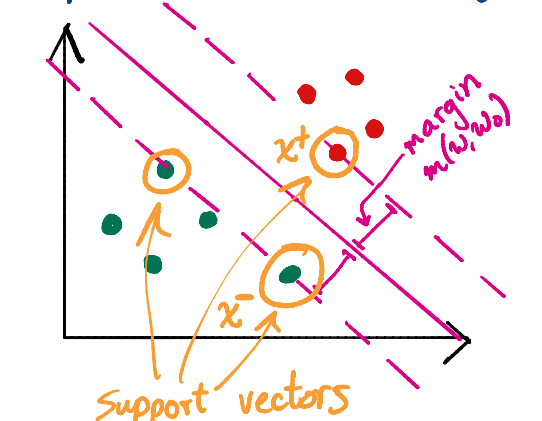
\includegraphics[width=0.6\columnwidth]{images/7-SVM-max-margin}
\end{center}

\textbf{Goal: }
\begin{equation*}
	\begin{gathered}
		\max_{\w, w_0} 2m(\w,w_0) \quad\textit{s.t.} \\
		\w^Tx_i + w_0 > 0 \iff y_i = +1 \\
		\w^Tx_i + w_0 < 0 \iff y_i = -1 \\
		\equiv y_i(\w^Tx_i + w_0) \geq b > 0
	\end{gathered}
\end{equation*}

\begin{align*}
	2m(\w, w_0) &= \norm{\textit{proj}_\w x^+ - \textit{proj}_\w x^-} \\
				&= \norm{\frac{\w^T x^+}{\norm{\w}^2} \w -\frac{\w^T x^-}{\norm{\w}^2} \w} \\
				&= \frac{1}{\norm{\w}} |\w^T x^+ - \w^T x^-|
\end{align*}

$m(\w, w_0)$ does not depend on $\norm{\w}$ nor $w_0$: Let $\gamma \in \R: $

$$
	m(\gamma \w, w_0) = \frac{1}{\gamma\norm{\w}} |\gamma\w^Tx^+ - \gamma\w^Tx^-| = m(\w, w_0)
$$

There is $w^*, w_0^*$ optimal such that $w^{*T}x^+ + w_o^* = 1$ and $w^{*T}x^- + w_0^* = -1$:

\begin{align*}
	2m(\w^*, w_0^*) &= \frac{1}{\norm{\w^*}} |\w^{*T}x^+ - \w^{*T} x^-| = \frac{2}{\norm{\w^*}}\\
	w^{*T}x_i + w_0^* &\geq w^{*T}x^+ + w_0^* = 1 \textit{ if } y_i = +1 \\
	w^{*T}x_i + w_0^* &\leq w^{*T}x^- + w_0^* = 1 \textit{ if } y_i = -1 \\
\end{align*}

\textbf{SVM formulation: } 
\begin{equation*}
	\begin{gathered}
		\min_{\mathbf w, w0}\frac{1}{2}\norm{\mathbf w}^2 \\
		\textit{s.t.}:  y_i(\mathbf w^T x_i + w_0) \geq 1
	\end{gathered}
\end{equation*}

\textbf{Slaters Condition}
\begin{itemize}
	\item By linear separation: $\exists \w, w_0: y_i(\w^T x_i + w_0)\geq 1, i\leq n$
	\item Take $\gamma>1 \implies (\gamma\w, \gamma w_0)$
	\begin{align*}
		y_i(\gamma\w^T x_i + \gamma w_0) &= \gamma y_i(\w^T x_i + w_0) \\
										&> y_i(\w^T x_i + w_0 \\
										&\geq 1
	\end{align*}
\end{itemize}


\textbf{Dual}
\begin{align*}
	\mathcal L(\w, w_0, \alpha) &= \frac{1}{2}\norm{w}^2 + \sum_i\alpha_i(1. yi(\w^Tx_i + w_0)), \alpha_i \geq 0 \\
	&= \frac{1}{2}\w^T\w + \sum_i\alpha_i \\
	&\quad\quad\quad- \sum_i\alpha_i y_i\w^Tx_i - \sum_i\alpha_i y_i w_0 \\
	\frac{\partial\mathcal L}{\partial \w} &= \w + 0- \sum_i\alpha_i y_i x_i + 0 \\
	\frac{\partial\mathcal L}{\partial w_0} &= 0 + 0 + 0 - \sum_i\alpha_i y_i
\end{align*}

Setting the derivatives to $0$ yields:
\begin{equation*}
	w^* = \sum_i\alpha_i y_i x_i, \quad \sum_i \alpha_i y_i = 0 
\end{equation*}
Plugging this into the dual formulation, we get:

\begin{equation*}
	\begin{gathered}
		\max_\alpha \frac{1}{2}\sum_{i,j} \alpha_i\alpha_jy_iy_jx_i^Tx_j + \sum_i \alpha_i - \sum_{i,j} \alpha_i\alpha_jy_iy_jx_i^Tx_j \\
		\alpha_i\geq 0, \sum_i\alpha_i y_i = 0
	\end{gathered}
\end{equation*}

which simplifies to
\begin{equation*}
	\begin{gathered}
		\max_\alpha \sum_i \alpha_i-\frac{1}{2}\sum_{i,j} \alpha_i\alpha_jy_iy_jx_i^Tx_j\\
		\alpha_i\geq 0, \sum_i\alpha_i y_i = 0
	\end{gathered}
\end{equation*}

\subsection{Shockfish}
Shockfish aims at predicting parking lot occupancy. Classification task: Occupied vs. non-occupied?

\textbf{Idea:}
\begin{itemize}
	\item Sense earth magnetic fields and measure deviations
	\item Deviations occur when a large mass (e.g. truck) is close to the sensor
	\item Sensor at each parking lot, use readings to detect presence of vehicle.
\end{itemize}

\textbf{Sensor Readings: }
\begin{itemize}
	\item Center Values: Temperature and other physical variations
	\item Data set: $\textit{signal}(t) = \textit{reading}(t) - \textit{center}(t)$
\end{itemize}

\textbf{Problem: }Truck also influences sensor measurements of neighboring sensors
\begin{itemize}
	\item[$\Rightarrow$] Weak coupling of neighboring sensors 
\end{itemize}

\subsubsection{Challenges}
\begin{itemize}
	\item Design new algorithm
	\item Label the readings of three weeks based on camera imagery
	\item find approp. data preprocessing filters
	\item Performance measures: Accuracy, Generalization (over sensors and parking lots).
	\item Have to carefully specify conditioning on sensor or parking lot.
\end{itemize}

\subsubsection{Problems in Real World Applications}
\begin{itemize}
	\item Non uniformity of sensors (not aligned, calibration errors, ...)
	\item Signals for occupied lots are not homogeneous (every truck generates different signal depending on steel mass and relative position)
\end{itemize}

\subsubsection{Data Preprocessing}
\textbf{Goal: } Fina transformation of the data such that the readings are as comparable as possible and the signal discriminability between occupied and non-occupied is maintained.

\textbf{Comparison of readings} when the entire lot is empty (rest readings) to compare different sensors.

\textbf{Preprocessing: }
\begin{enumerate}
	\item Center Values
	\item Subtract median of rest readings per sensor
	\item Subtract minimal rest readings accross sensors
	\item Transform to spherical coordinates
\end{enumerate}

\subsubsection{Modeling: Classify parking space occupancy}
\textbf{Types of information: } Spatial (individual sensors, neighborhood), transition information (changes between consecutive readings)

\textbf{Classifiers: } SVM, Random Forest, Graphical Models

\textbf{Features: }
\begin{itemize}
	\item Measurements (Z-axis informative, X-axis not informative)
	\item Spherical coordinates: $r$ very informative, angles exhibit high variations in consecutive readings in the non occ. state
	\item Time of the day (likelihood varies)
\end{itemize}		
	\section{SVMs for non-linear Classification}
\textbf{Solutions for not linearly separable training sets:}
\begin{itemize}
	\item Soft-margin SVM
	\item Kernels
\end{itemize}


\subsection{Soft-Margin SVMs}
Train a max-margin classifier (see Section 7), but neglect some samples.
\begin{equation*}
	\begin{gathered}
		\min_{\w, w_0} \frac{1}{2}\norm{\w}^2 + C\sumin\xi_i \\
		\textit{s.t.}\quad y_i(\w^Tx_i + w_0) \geq 1 - \xi_i, \xi_i \geq 0
	\end{gathered}
\end{equation*}
Tradeoff: wide. margin $C$ = many samples neglected, narrow margin= few samples neglected. $\xi_i$ lowers the bar for each neglected example.

\textbf{Dual: }
\begin{equation*}
	\begin{gathered}
		\max_\alpha \sum_i - \frac{1}{2}\sum_{i, j}\alpha_i\alpha_j y_i y_j x_i^Tx_j \\
		\textit{s.t.} \quad 0\leq \alpha_i\leq C, \sum_i\alpha_i y_i = 0
	\end{gathered}
\end{equation*}

\textbf{Optimum: }
\begin{align*}
	w^* &= \sum_i \alpha_i^* y_ix_i \\
	\xi_i^*	&= \max(0, 1-y_i(w^{*T} x_i + w_0^*))
\end{align*}


\subsection{Kernels}
Kernels transform the data from a not linearly separable space to a linearly separable space.

\textbf{Polynomial Transformation: }
$$
	\varphi: (t,c) \mapsto (1, t, c, t^2, c^2, tc, t^3, t^2c, tc^2, c^3, ...)
$$
Using this, we can go from polynomial classification to linear classification: 
$$
	\sumj{\infty}\sum_{n_1 + n_2 = j} w_{n.n_2}t^{n_1}c^{n_2} = w_00 + w_1t + w_2c + ... = w^T\varphi(t,c)
$$

\subsubsection{SVMs and kernels}
\begin{enumerate}
	\item Training: 
	\begin{equation*}
		\begin{gathered}
			\max_\alpha \sumin\alpha_i - \frac{1}{2}\sum_{i,j}\alpha_i\alpha_jy_iy_j {\color{imp} \varphi(x_i)^T\varphi(x_j)} \\
			\textit{s.t.} \quad 0\leq \alpha_i\leq C, \sum_i\alpha_i y_i = 0
		\end{gathered}
	\end{equation*}
	\item Classification:
	\begin{equation*}
		w^{*T} \varphi(x) = \left(\sum_i \alpha_i^*y_i\varphi(x_i)\right)^T\varphi(x) = \sum_i \alpha_i^*y_i\varphi(x_i)^T\varphi(x)
	\end{equation*}
\end{enumerate}

We do not need $\varphi(x_i)$ or $\varphi(x)$. We just need $\varphi(x_i)^T\varphi(x)$.


\subsubsection{Important Kernels}
\begin{equation*}
	\begin{gathered}
		\mathcal K: \mathcal X \times \mathcal X \to \R \\
		(x,y) \mapsto \varphi^T(x) \varphi(y)
	\end{gathered}
\end{equation*}

\begin{align*}
	\K(x,y) &= \exp(-\gamma\norm{x-y}^2) & \textit{RBF-kernel} \\
	\K(x,y) &= \tanh(\gamma x y ) - b & \textit{sigmoid }\\
	\K(x,y) &= (x^Ty)^d & \\
	\K(x,y) &=	(x^Ty + 1)^d & 
\end{align*}
(RBF = radial-basis function)

\subsubsection{Kernel engineering}
if $k_1, k_2$ are valid kernels,$c>0$, $q$ polynomial, $f$ function, $\phi: \mathcal X \to \R^m$, $A$ symmetric and pos. sem. def. Then the following are also valid kernels:

\begin{multicols}{3}
	$ck_1(x,x')$ \\ $f(x) k_1(x,x')f(x')$ \\ $q(k_1(x,x')$ \\ $\exp(k_1(x.x')$
	$k_1(x,x') + k_2(x,x')$ \\ $k_1(x,x')k_2(x,x')$ \\ $k_3(\phi(x), \phi(x'))$ \\ 
	$x^TAx'$ \\ $k_a(x_a, x_a')k_b(x_b, x_b')$ \\ $k_a(x_a, x_a') +\\ k_b(x_b, x_b')$
\end{multicols}

\subsubsection{Mercer's Theorem: }
$\K: \mathcal X \times \mathcal X \to \R$

If $\K(x,y) = \K(y,x)$ and $\int\int f(x) \mathcal K(x,y)f(y) dxdy \geq 0$ for any $f\in L^2$, then $\K$ is a Kernel.



\subsection{Structural SVMs}
Structural SVMs can be seen as a generalization of SVM, where we can predict general structured output
\subsubsection{Multi-Class Classification}
One-vs-rest classification: $c(x) =\arg\max_y \text{score}_y(x)$

We can't do this for structural SVMs: there are too many classes and no inter-class learning.

\subsubsection{Joint feature maps: }
\begin{equation*}
	\begin{gathered}
		\Psi: \mathcal X \times \mathcal Y \to \R^m \times \mathbb Z^n \\
		\Psi(\textit{"the dog chases the cat"}), \langle \textit{tree structure} \rangle) \mapsto w
	\end{gathered}
\end{equation*}
\begin{itemize}
	\item One weight vector for all classes
	\item $\w^T\Psi(x,y) = \textit{compatibility score between $x$ and $y$}$
	\item $c(x) = \arg\max_y \w^T\Psi(x,y)$
\end{itemize}
\textbf{SVM formulation: }
We do not want to require the same "gap" for all pairs of classes (make a difference between small and large mistakes: $\Delta(y,y')\in \R^+$)

\begin{equation*}
	\begin{gathered}
		\min_w \frac{1}{2} \norm{w}^2 \\
		\textit{s.t. } w^T\Psi(x_i, y_i) \geq {\color{imp}\Delta(y_i, y')} + w^T\Psi(x_i, y') \\
		\forall y'\neq y_i, i\leq n
	\end{gathered}
\end{equation*}
\textbf{Loss function: }
\begin{center}
	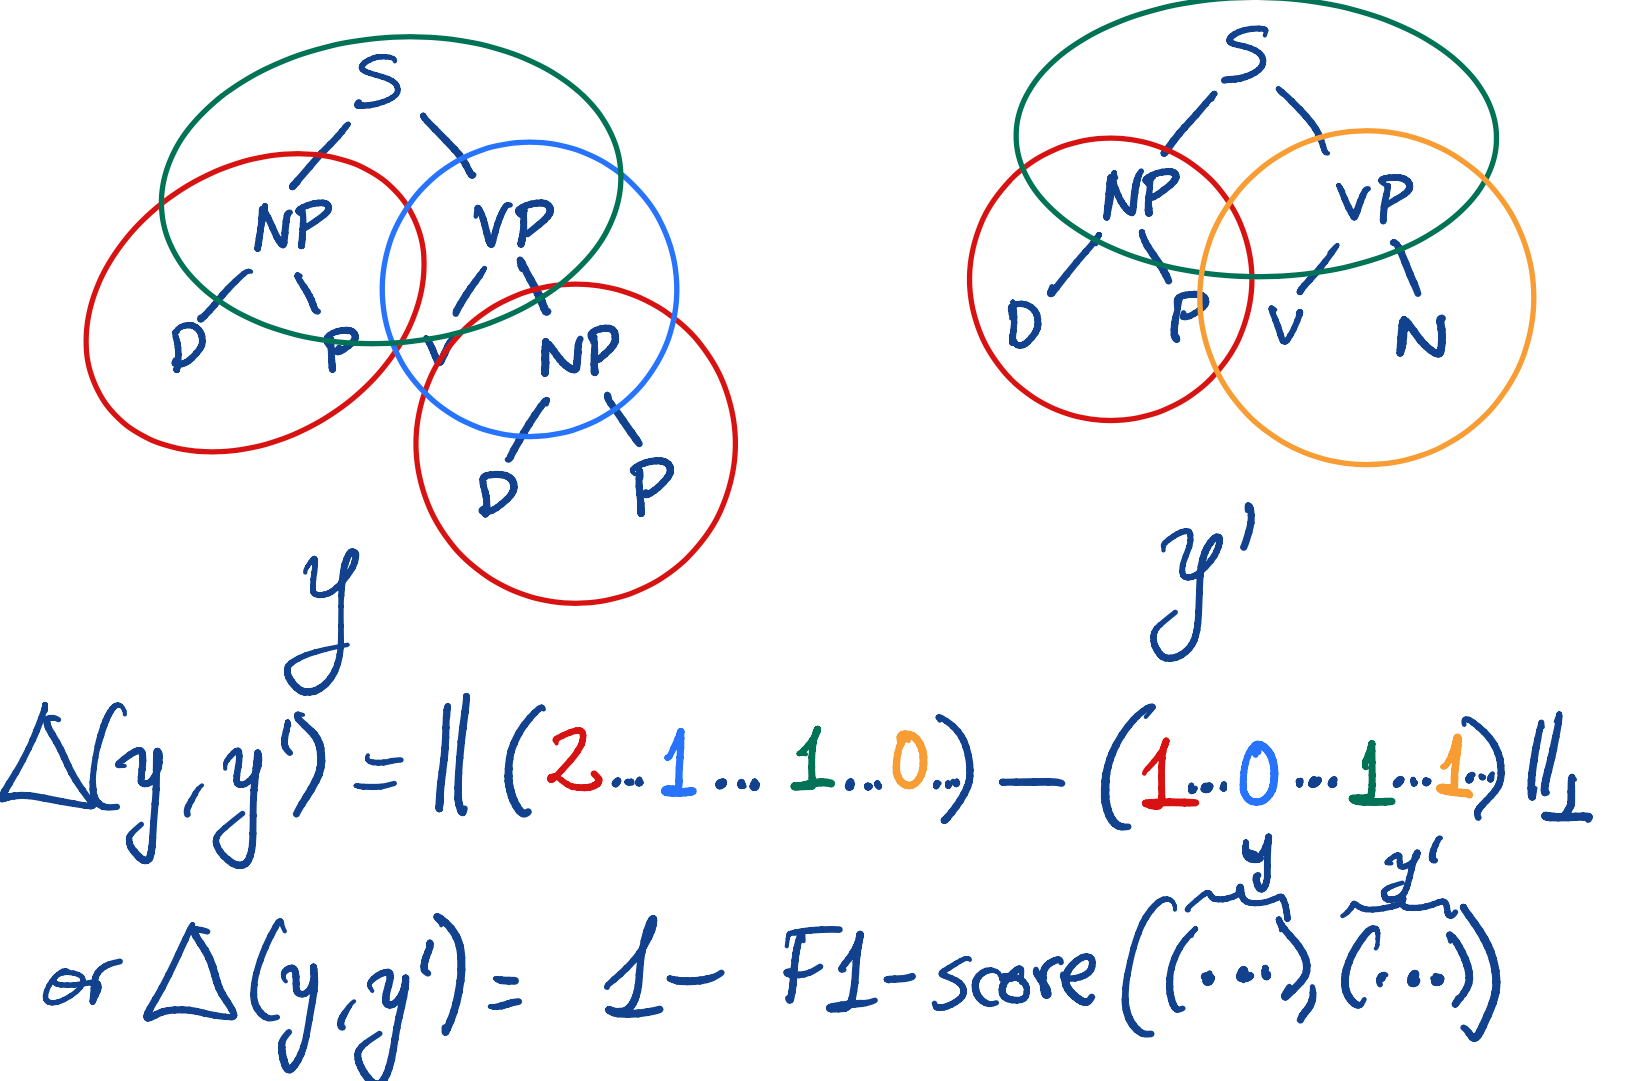
\includegraphics[width=.7\columnwidth]{images/8-ssvm-joint-feature-maps.png}
\end{center}

\textbf{Soft-margin Formulation}
\begin{equation*}
	\begin{gathered}
		\min_{w,\xi} \frac{1}{2} \norm{w}^2 + {\color{imp} \frac{C}{{\color{imp2}n}}\sumin \xi_i} \\
		\textit{s.t. }  w^T\Psi(x_i, y_i) \geq \Delta(y_i, y') + w^T\Psi(x_i, y') - {\color{imp} \xi_i} \\
		\xi_i \geq 0, \forall y'\neq y_i, i\leq n
	\end{gathered}
\end{equation*}
\textbf{Why the {\color{imp2}n}?}

Theorem: If $w^*. \xi^*$ are optimal, then the empirical risk of $w^*$ w.r.t $\Delta$ is 
\begin{align*}
	\E_{x,y}[\Delta (Y, c_w(x))] 	&= \frac{1}{n}\sumin\Delta(y_i, c_w(x_i)) \\
									&\leq \frac{1}{n} \sumin\xi_i
\end{align*} 
\textit{Proof on slide 42}

The conditions can also be written as: 
\begin{equation*}
	\begin{gathered}
		\textit{s.t. }  w^T\Psi(x_i, y_i) \geq 1 + + w^T\Psi(x_i, y') - \frac{{\color{imp} \xi_i}}{\Delta(y_i, y')} \\
		\xi_i \geq 0
	\end{gathered}
\end{equation*}
This formulation is \textbf{invariant to rescaling of $\mathbf \Delta$}




\subsubsection{Training Algorithm}
\begin{algorithm}[H]  
	\SetKwInOut{Input}{input}
	\Input{tolerance threshold $\epsilon > 0$}
	$\w\gets 0, \xi\gets 0, W\gets \emptyset$ \\
   \DoUntil{$W$ does not change}
   {
   		\For{$i\leq n$}
   		{
			$y'\gets \arg\max_{y\neq y_i} \left\{ \Delta(y_i, y) + w^T\Psi(x_i, y)\right\}$ 
			
			\If{$(w^T\Psi(x_i, y_i)$ $\not\geq$ $\Delta(y_i, y') + w^T(x_i, y') - \xi_i-\epsilon)$}{
				$ W\gets W \cup \left\{w^T\Psi(x_i, y_i) \geq \Delta(y_i, y') -\xi_i + w^T\Psi(x_i, y') \right\}$
			}      		
      	}
      	$w, \xi \gets \textit{solve}\left(\min_w \frac{1}{2} \norm{w}^2 + \frac{C}{n} \sum_i\xi_i \textit{ s.t. } W \right)$
  	}
  \caption{SVM training algorithm}
\end{algorithm}
	
\subsubsection{Prediction: }
$$
	c(x) = \arg\max_y w^T\Psi(x,y)
$$

\subsection{Advantages and Disadvantages}
\begin{center}
	\begin{tabular}{ p{0.45\columnwidth} | p{0.45\columnwidth} } 
		\textbf{Advantages} & \textbf{Disadvantages}\\\hline
			- Works well with infinitely dimensional representations & - requires careful model selection \\
			-  Adapted to structured classification & - Requires feature Engineering \\
			- Formulated as QP, for which efficient procedures are available & - Use of kernels make training algos succeptible to curse of dim
	
	\end{tabular}
\end{center}

\textit{Examples on page 51 - 64 (page ranking, diseases, ...)}
	
	
			
	\section{Ensemble Methods}
\begin{highlight}{Bagging vs. Boosting}
\begin{tabular}{ p{0.45\columnwidth} | p{0.45\columnwidth} }
		\textbf{Bagging} & \textbf{Boosting}\\\hline
		 trains learners in parallel and combines them using deterministic averaging. & trains learners sequentially in an adaptive way and combines them using a deterministic strategy. \\\hline
  		 less variance than the components & less biased than the components 
\end{tabular}



\end{highlight}
Combination of multiple weak learners to get a stronger learner. (Wisdom of crowds)
\subsection{Bagging}
\begin{enumerate}
	\item Bootstrap sets: Draw $M$ bootstrap sets
	\item Train $M$ base models $b^{(1)}, ... , b^{(M)}$
	\item Aggregate 
	$$	\bbar =
		\begin{cases}
			\frac{1}{M}\sum_{t\leq M} b^{(t)}(x) &\text{regression}\\
			\textit{majority}\left(b^{(t)}(x)\right)_{t\leq M}&\text{classification}
		\end{cases}
	$$
\end{enumerate}
\begin{center}
	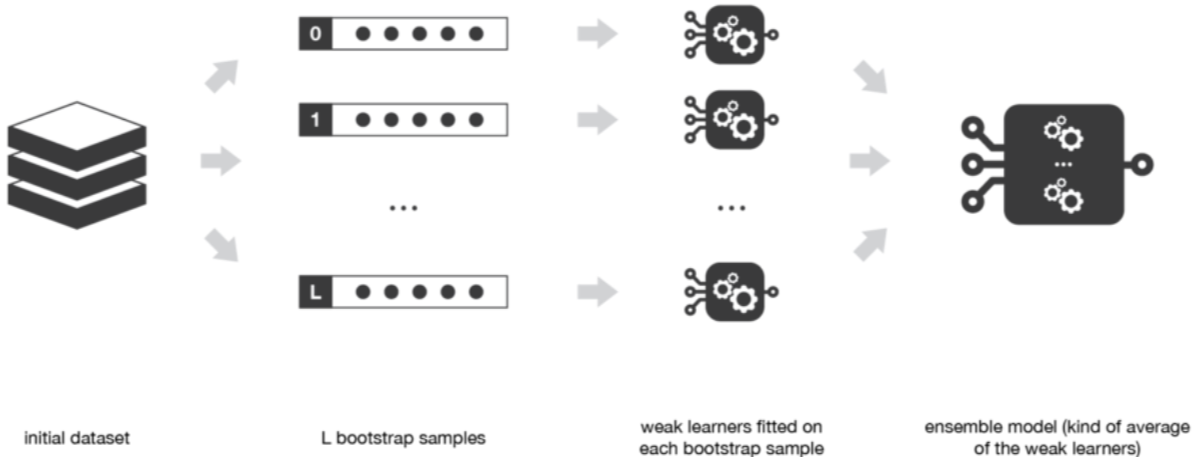
\includegraphics[width=\columnwidth]{images/9-bagging}
\end{center}

\textbf{Theorem}: For $x\in \mathcal X$ if $range(y) < \infty$, then there is a sufficiently large $M$ s.t. $\E[(y - \bar{b}^{(M)}(x))^2] \leq \E[(y - b(x))^2]$ for some base model $b$.

\textit{Proof in Slides, p.20-21}


\textbf{Properties of the base models}
\begin{itemize}
	\item Diversity
	\item Independence: Bootstrap sets should be independent, but \textbf{they are not} (but correlation is small).
\end{itemize}



\subsubsection{Random forests}
\textit{The \href{https://towardsdatascience.com/ensemble-methods-bagging-boosting-and-stacking-c9214a10a205}{Random forest} method is a bagging method with trees as weak learners. Each tree is fitted on a bootstrap sample considering only a \textbf{subset of variables} randomly chosen. This helps \textbf{reduce the correlation} between trained base trees in the ensemble.
}
\begin{center}
	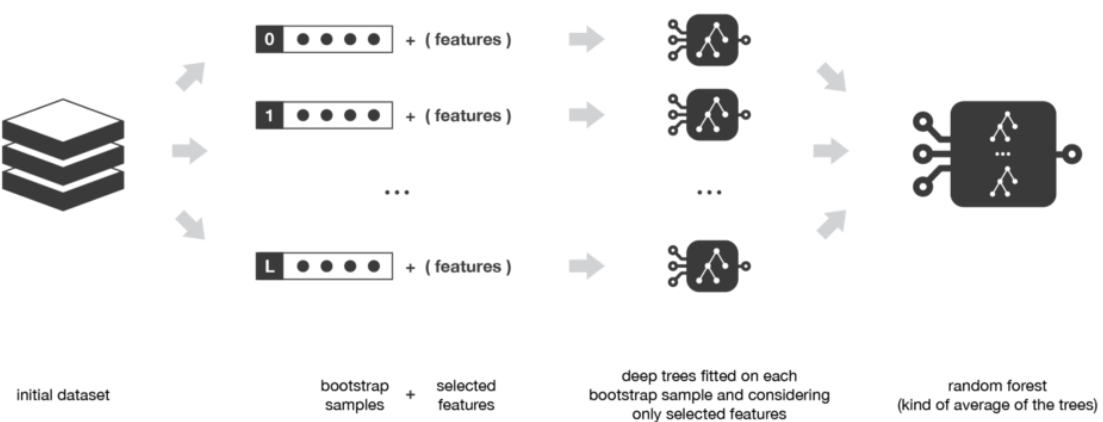
\includegraphics[width=\columnwidth]{images/9-random-forests}
\end{center}





\subsection{Boosting }
\textit{Key: Learning from previous mistakes.}

Fit models iteratively, such that the training of the model at a given step depends on the models fitted in previous steps. Each model gives higher weight to the observations that were handled badly in the previous steps.


\begin{center}
	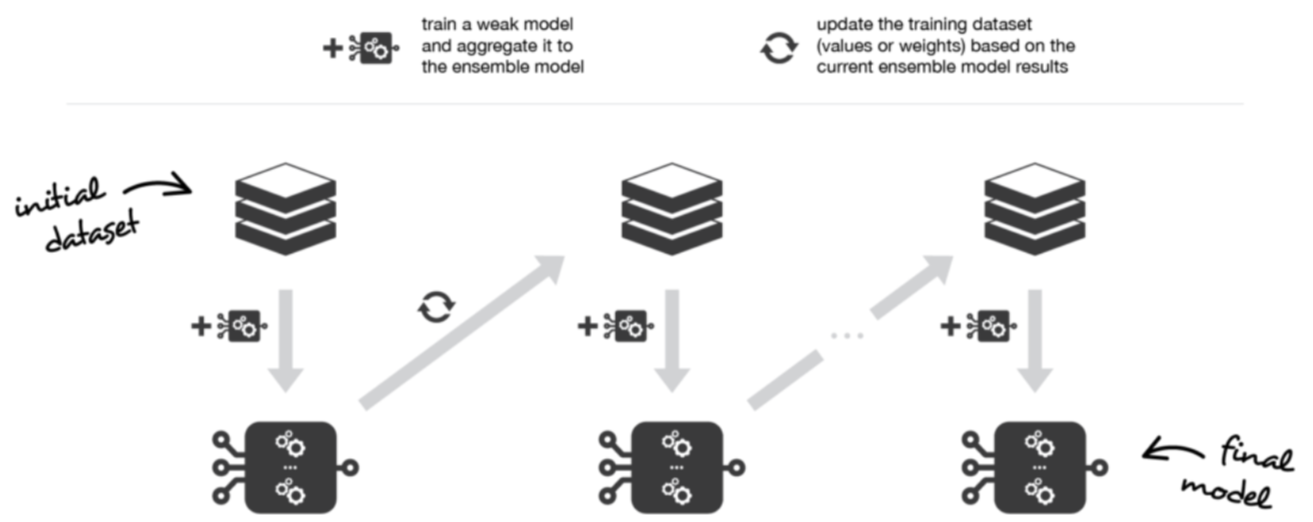
\includegraphics[width=0\columnwidth]{images/9-boosting}
\end{center}


\subsubsection{Ada Boost (Adaptive Boosting)}
\textit{Learn from previous mistakes by increasing the weight of misclassified datapoints. \textbf{Outliers} will get very high weights and can be detected by that.
}\begin{itemize}
	\item Loss function: $0$-$1$ Loss
	\item Base models (stumps)
	\item place high weights on samples that are very hard to classify
\end{itemize}



Let $\mathcal L^{(w)} = \sumin w_i * \mathds{1} \{b(x_i)\neq y_i\}$ (the 0-1 loss)

\begin{algorithm}[H]  
	\tcp{Initialize}
	$\bbar^{(0)} \gets 0$ \\ 
	$w_i \gets 1/n$ for $i\leq n$ \\
	\For{t=1..M}{
		\tcp{Train}
		$b^{(t)} \gets \arg\min_b \L^{(w)}(b)$\\ 
		\vspace{1em}
		\tcp{Evaluate}
		$err_t \gets \mathcal L^{(w)}(b^{(t)})$\\
		\vspace{1em}
		\tcp{Reweigh}
		$w_i \gets
			\begin{cases}
				\tilde\alpha_tw_i &\textit{if }b^{(t)}(x_i)\neq y_i \textit{ for } i\leq n, \tilde\alpha_t = \frac{1}{err_t}-1 \\
				w_i &\textit{otherwise }
			\end{cases}$ \\
		\vspace{1em}
		\tcp{Add to set}
		$\bbar \gets \bbar^{(t-1)} + \tilde \alpha_t b^{(t)}$\\
		\vspace{1em}

		\textit{normalize}($ w_1, ... ,w_n$)\\
	}
	\caption{AdaBoost Algorithm}
\end{algorithm}


\textbf{AdaBoost for Classification: } 
\begin{enumerate}
	\item Train $\alpha_1, b^{(1)}, ..., \alpha_M, b^{(M)}$
	\begin{equation*}
		\begin{gathered}
					\alpha_1, b^{(1)}, ..., \alpha_M, b^{(M)} \\
			\alpha_t \in [0, \infty) \\
			b^{(t)}: \mathcal X \to \{-1, +1\}
		\end{gathered}
	\end{equation*} 
	\item predict $\bbar^{(M)} = sgn(\sum_{t\leq M}\alpha_tb^{(t)}(x))$
\end{enumerate}

\textbf{Why is AdaBoost so successful?}
\textit{Theoretical results: Slides p. 57-}
\begin{itemize}
	\item Friedmann: AdaBoost is equal to forward additive stepwise modeling (FSAM) with exponential loss
		\item Boosting trains max-margin classifiers
	\item Wyner et al: AdaBoost and random forest train spiky, interpolating and self-averaging models.
	
	\begin{minipage}{0.35\columnwidth}
	\textbf{Spiky: }
	\begin{center}
		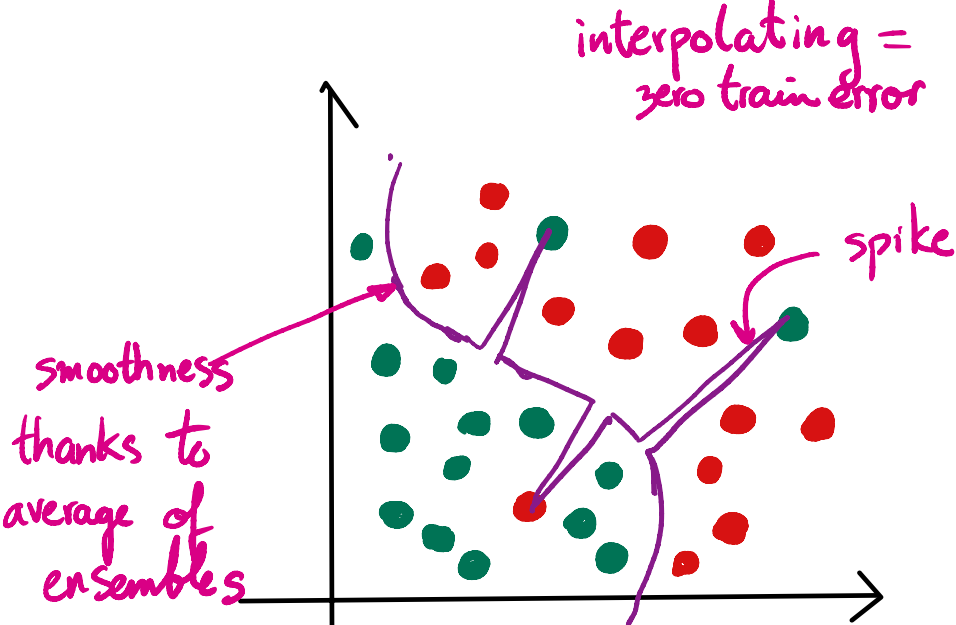
\includegraphics[width=\columnwidth]{images/9-adaboost-spiky}
	\end{center}
	\end{minipage}
	\begin{minipage}{0.55\columnwidth}
		\begin{itemize}
			\item Mostly smooth with Sharp localized changes to interpolate noisy examples
			\item This prevents influence from noise and allows fitting of complex signals.
		\end{itemize}
	\end{minipage}
	
	\begin{minipage}{0.35\columnwidth}
	\textbf{Self-Averaging: }
	\begin{center}
		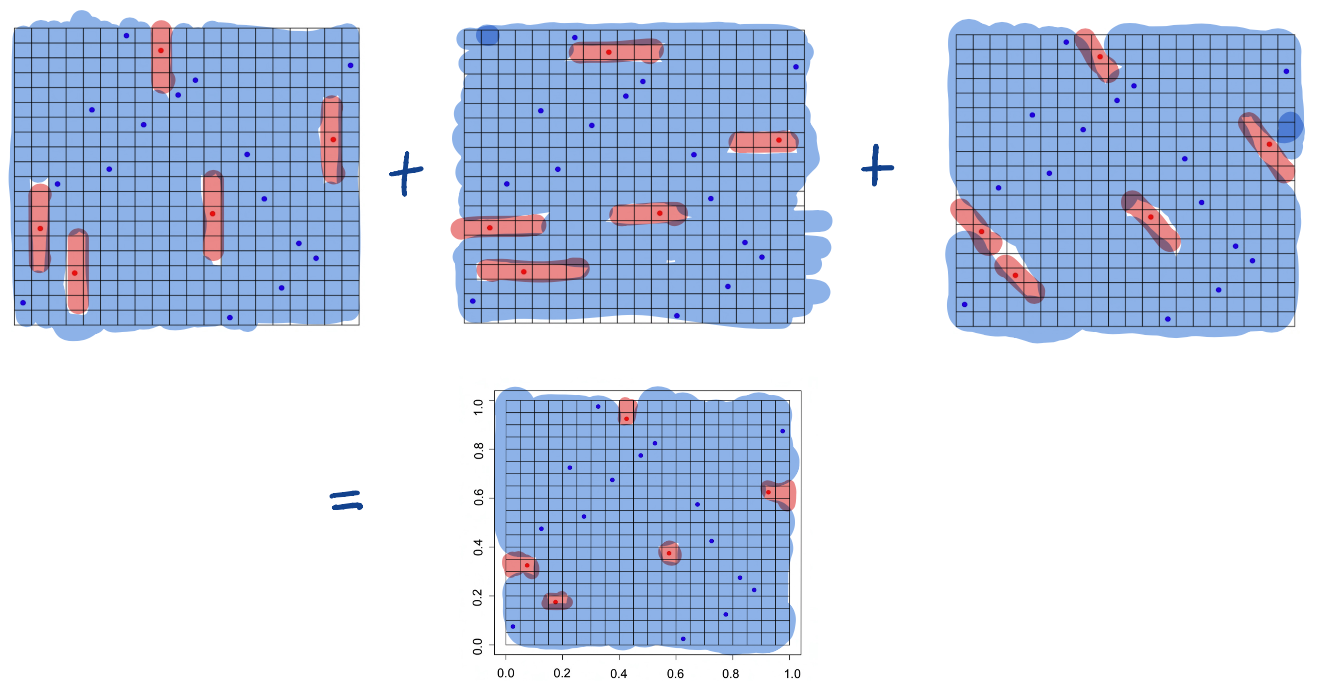
\includegraphics[width=\columnwidth]{images/9-adaboost-selfavg}
	\end{center}
	\end{minipage}
	\begin{minipage}{0.55\columnwidth}
		\begin{itemize}
			\item Trained model is an average of diverse models
			\item Averaging spiky interpolation helps localise noisy effects
		\end{itemize}
	\end{minipage}	
\end{itemize}

\begin{minipage}{\columnwidth}
	\textbf{AdaBoost with complex base classifiers trains spiky interpolation classifiers.}



\begin{tabular}{p{0.2\columnwidth} | p{0.2\columnwidth} | p{0.2\columnwidth} | p{0.2\columnwidth}}
		\textbf{base classif.} & \textbf{Vertical Stumps} & \textbf{Stumps} & \textbf{Full Trees}\\\hline
		\textbf{Trained Ensemble}
		&
  		\begin{center}
  		\vspace{-1em}
			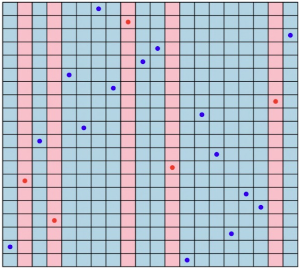
\includegraphics[width=0.2\columnwidth]{images/9-adaboost-baseclassif-1}
		\end{center} &  
		\begin{center}
  		\vspace{-1em}
			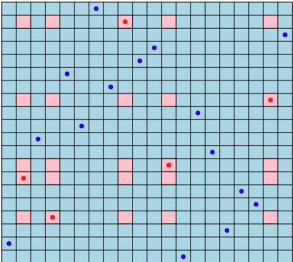
\includegraphics[width=0.2\columnwidth]{images/9-adaboost-baseclassif-2}
		\end{center}
  		& 
  		\begin{center}
  		\vspace{-1em}
			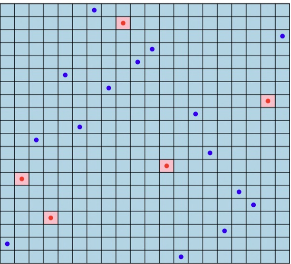
\includegraphics[width=0.2\columnwidth]{images/9-adaboost-baseclassif-3}
		\end{center} \\\hline
		\textbf{gen. error} & high & medium & low \\\hline
		\textbf{Interp.} & $\checkmark$ & $\checkmark$ & $\checkmark$ \\\hline
		\textbf{spiky} & $\times$ & $\sim$ & $\checkmark$ \\\hline
\end{tabular}
\end{minipage}

\subsubsection{Gradient Boosting}
\textit{Similarly to AdaBoost, gradient Boosting is a\textbf{ method to greedily approximate $f$} using gradient descent based on the additive form. Gradient Boosting learns directly from the residual error instead of updating the weights. }
\begin{equation*}
	f_M(x) = \sumi M \beta_i h_i(x), \textit{where $h_i$ are the weak learners.}
\end{equation*}

\begin{algorithm}[H]  
	$\hat f_0(\x) = \argmin_h \sumi n L(y_i, h(\x_i)$\tcp*[r]{Init}
	\For{t=1..M}{
	\tcp{Compute the negative gradient :} 
		$-g_m(\x_i) = \left[\frac{\partial L(y_i, f(\x_i))}{\partial f(\x_i)} \right]_{f = \hat f_{m-1}(\x_i)}, i= 1... n$ \\\vspace{1em}

		\tcp{Fit function $h_m$ to negative gradient by least squares: } 
		$h_m = \argmin_h\sumi n(-g_m(\x_i - h(\x_i))^2$ \\\vspace{1em}

		\tcp{Find $\beta_m$ to minimize the loss } 
		$\beta_m = \argmin_\beta\sumi n L(y_i, \hat f_{m-1}(\x_i) - h(\x_i))^2$\\\vspace{1em}
		
		\tcp{Update $\hat f$} 
		$\hat f_m(\x) = \hat f_{m-1} + \beta_mh_m(\x)$
	}
	\caption{Gradient Boosting algorithm}
\end{algorithm}

\textbf{Differences AdaBoost / Gradient Boosting: }
\begin{itemize}
	\item AdaBoost learns from mistake by increasing the weight of misclassified data-points.
	\item Gradient Boosting learns from the residual error (mistake) directly instead of updating weights.
\end{itemize}


\subsubsection{Forward Stagewise Additive Modeling (Exercise 6)}
Method to approximately compute a classifier of the form $c(x) = \mathit{sgn}(\sum_t\alpha_t b^{(t)}$ that approximately minimizes the empirical loss $\sumin L(y_i, c(x_i))$.

\begin{algorithm}[H]  
	\SetKwInOut{Input}{input}
	\SetKwInOut{Output}{output}
	
	\Input{
		\begin{itemize}
			\item $\{(x_1, y_1), ..., (x_n, y_n)\}\subseteq\R^D\times \{-1, 1\}$
			\item $L:\{1, -1\}\times \{1, -1\}\to \R$
			\item $M\in \N$
		\end{itemize}
	}
	\Output{$\hat c \approx \argmin_c \sumi n L(y_i, c(x_i))$} 
	\vspace{1em}
	
	$f_0(x) \gets 0 \forall x\in\R^D$ \\
	\For{$t=1$ to $M$}{
		$(\alpha_t, b^{(t)}) \gets \argmin_{\substack{\alpha > 0 \\ b\in\mathcal H}} \sumi n L(y_i, \alpha b(x_i) + f_{t-1}(x_i))$ \\
		$f_t(x) \gets \alpha_tb^{(t)}(x) + f_{t-1}(x) \forall x\in\R^D$ \\
	}
	\Return{$\hat c \gets \mathit{sgn}(f_M(x)) \forall x\in\R^D$}
	\caption{Forward stagewise additive modeling}
\end{algorithm}

$\Rightarrow$ \textbf{Exercise 1: AdaBoost is equivalent to forward stagewise additive modeling}
	
	\section{Deep Learning}
\subsection{Feed-Forward Neural Networks}
\textit{Function that applies linear transformation and activation functions.}

\begin{itemize}
	\item (L)inear functions $L: x\mapsto Wx + b$
	\item ($\alpha$)ctivation function: $\alpha: x \mapsto (\alpha(x_1), ..., \alpha(x_n))$
\end{itemize}

\begin{align*}
		\NN(x) 	&= \ap d (\Lp d (...\ap 2(\Lp 2((\ap 1(\Lp 1)))))) \\
				&= \ap d \circ \Lp d \hdots \ap 2 \circ \Lp 2 \circ \ap 1 \circ \Lp 1(x)
	\end{align*}

\subsubsection{Activation Functions}
\textit{Activation functions make the NN function non-linear.
}\vspace{1em}

\begin{minipage}{0.45\columnwidth}
\textbf{ReLu}: 
$$
	f(x) = \begin{cases}
		0 &\textit{for $x<0$} \\
		x &\textit{for $x\geq 0$}
	\end{cases}
$$
Danger of vanishing gradient on the left.
\end{minipage}
\begin{minipage}{0.4\columnwidth}
	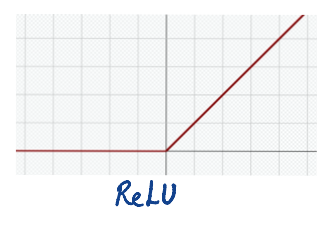
\includegraphics[width=\columnwidth]{images/10-relu}
\end{minipage}

\begin{minipage}{0.45\columnwidth}
	\textbf{Sigmoid}: 
$$
	\sigma(x) = \frac{1}{1 + \exp(-x)}
$$
Danger of vanishing gradient on both sides.
\end{minipage}
\begin{minipage}{0.4\columnwidth}
		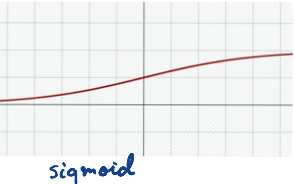
\includegraphics[width=\columnwidth]{images/10-sigmoid}
\end{minipage}

\begin{equation*}
	\sigma'(x) = 
	\begin{cases}
		\sigma(x)(1-\sigma(x)) &\textit{if dim$(x) = 1$} \\
		\sigma(x)\circ(1-\sigma(x))  &\textit{if dim$(x) > 1$}
	\end{cases}
\end{equation*}


\begin{minipage}{0.45\columnwidth}
	\textbf{Tanh}: 
$$
	\tanh(x) = \frac{2}{1 + e^{-2x}}-1
$$

Danger of vanishing gradient on both sides
\end{minipage}
\begin{minipage}{0.4\columnwidth}
		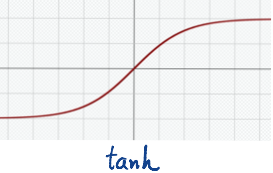
\includegraphics[width=\columnwidth]{images/10-tanh}
\end{minipage}
\vspace{1em}

\textbf{Theorem Cybenko:}\\
If $f: [0,1]^n\to\R$ is continuous, $\epsilon > 0$, then there is a neural net s.t.
\begin{enumerate}
	\item $\NN(x) = \sumim \alpha_i\sigma(w_i^Tx + b_i)$
	\item $\max_x |f(x) - \NN(x)| < \epsilon$ 
\end{enumerate}
\vspace{1em}

\textbf{Pooling Layers: } average the results from previous layer. \\
\textbf{Output Layers: }
\begin{itemize}
	\item Binary classifier: One output, $\sigma(z)$ (sigmoid)
	\item Multi-Class: Soft-max layer to get probabilities from scores: 
	\textit{"Winner takes it all"}
	$$
		y_i= \frac{\exp)\beta z_i)}{\sum_{j\leq 3}\exp(\beta z_j)t}
	$$
	
\end{itemize}
\vspace{1em}
\textbf{Training Neural Networks}
\begin{equation*}
	\min_\theta \underbrace{\sumin \L(y_i, \NN_\theta(x_i))}_{\L(\theta)}, \quad \theta = (\weight{ 1}; b^{(1)}; \weight{2}; b^{(2)}, ....),
\end{equation*}

where $\theta$ are the parameters of the neural network.This function is analytically intractable, but easy to differentiate.

\vspace{1em}
\textbf{Forward propagation: }
$$
	a^{(l)} = \sigma(Wa^{(l-1)} + b)
$$
\textbf{Back-propagation: }\\
\textit{The only purpose of back-propagation is to compute the gradients $\frac{\partial\NN}{\partial w^l}$(not optimize them, that is what optimizers are for).}
\begin{itemize}
  \item Start at the output and propagate backwards, updating weights and biases for each layer.
  \item For wach layer, back propagate the weights and biases using back-propagation algorithm: 
\end{itemize}

$$
\frac{\partial C}{\partial w^l} = \frac{\partial C}{\partial z^L} \prod_{i=L...l+1}\left(\frac{\partial z^i}{\partial a^{i-1}}\frac{\partial a^{i-1}}{\partial z^{i-1}}\right)\frac{\partial z^l}{\partial w^l},
$$
where $L$ last layer, $z$ value before activation function, $a$ value after activation function.


\begin{highlight}{Backpropagation in Multi-Layer Perceptron (Assignment 7, Ex. 1)}
\begin{minipage}{0.5\columnwidth}
	To compute the values for backpropagation, we use the chain rule.
\begin{align*}
	\frac{\partial C}{\partial \weight{l}_r} &= \frac{\partial C}{\partial\nnout{l}}\frac{\partial \nnout{l}}{\partial\weight{l}_r} \\
	\frac{\partial C}{\partial \bias{l}} &= \frac{C}{\partial\nnout{l}}\frac{\partial \nnout{l}}{\partial\bias{l}} 
\end{align*}	
For example, we got:
	$$
		\frac{\partial C}{\partial\nnout{L}} = \frac{\partial C}{\partial \activation{L}}\frac{\partial \activation{L}}{\partial\nnout{L}}
	$$

Computing and substituting all of these values will result in the iteration step of stochastic gradient descent to update the weights matrix $\weight{l}_t$ and the biase vectors $\bias{l}_t$ as
\begin{align*}
	\weight{l}_t &= \weight{l}_{t-1} - \eta \frac{\partial C}{\partial \weight{l}} \\
	\bias{l}_t &= \bias{l}_{t-1} - \eta\frac{\partial C}{\partial \bias{l}}
\end{align*}

where
$\weight{l}_t$ is the $t$-th row of the weight matrix $\weight{l}$ and $C$ is the cost of the last layers output (i.e. $\L$)
\end{minipage}
\begin{minipage}{0.5\columnwidth}
	\begin{flushright}
		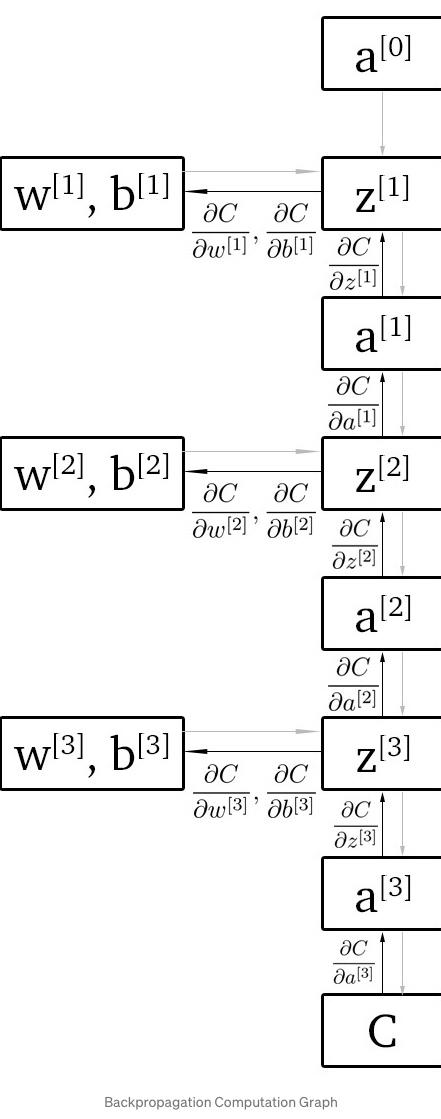
\includegraphics[width=0.8\columnwidth]{images/10-backpropagation}
	\end{flushright}
\end{minipage}
\end{highlight}

\subsubsection{Gradient Descent}
\begin{algorithm}[H]  
	$k\gets 0$ \\
	$\weight{k}_r \gets$ Unif$([-\sqrt{\frac{1}{n}}, \sqrt{\frac{1}{n}}])$ for $\l \leq d, r\leq$\#rows $W^{(l)}$ \\
   \DoUntil{\textit{difference between test-cost and train-cost starts increasing}}
   {
      $w^{(k+1)} \gets w^{(k)} - \eta(k)\nabla_{\weight l_r} \L(\theta)$ for $\l \leq d, \forall r $
      
      $k\gets k+1$ 
  	}
  \caption{General Form of Gradient Descent}
\end{algorithm}

%\begin{highlight}{How to compute $\nabla_{\weight{l}_r} \L(\theta)$}
%	\begin{enumerate}
%		\item Jacobian matrix: $\left(\frac{\partial F_i}{\partial w_j} \right)_{\substack{i\leq n\\ j\leq m}} : \R^m\to\R^{n\times m}$
%		\item Use the chain rule
%	\end{enumerate}
%	\todo[inline]{TODO: How is it done + example!}
%\end{highlight}

\begin{algorithm}[H]  
	$k\gets 0$ \\
	$\weight{k}_r \gets$ Unif$([-\sqrt{\frac{1}{n}}, \sqrt{\frac{1}{n}}])$ for $\l \leq d, r\leq$\#rows $W^{(l)}$ \\
   \RepeatUntil{\textit{...}}
   {
      do fwd and back propagation to compute $\frac{\partial \NN}{\partial\weight{l}_r} \vert_{\theta, x_i} $ for each $l,r,i\leq n$ \\
      $\frac{\partial\L}{\weight{l}_r} =\sumin \frac{\partial \L(y_i, \NN_\theta(x_i))}{\partial \weight{l}_r}$ \\
      $\weight{l}_r \gets \weight{l}_r - \eta(k) \frac{\partial \L}{\partial\weight{l}_r}$
  	}
  \caption{Gradient Descent}
\end{algorithm}

\begin{algorithm}[H]  
	$k\gets 0$ \\
	$\weight{k}_r \gets$ Unif$([-\sqrt{\frac{1}{n}}, \sqrt{\frac{1}{n}}])$ for $\l \leq d, r\leq$\#rows $W^{(l)}$ \\
   \RepeatUntil{\textit{...}}
   {
      do fwd and back propagation to compute $\frac{\partial \NN}{\partial\weight{l}_r} \vert_{\theta, x_i} $ for each $l,r,$ {\color{imp}$i\in S$, where $S$ is a sample from $\{1...n\}$} \\ 

      $\frac{\partial\L}{\weight{l}_r} =\sumin \frac{\partial \L(y_i, \NN_\theta(x_i))}{\partial \weight{l}_r} {\color{imp}\approx \sum_{i\in S}\frac{\partial \L(y_i, \NN_\theta(x_i))}{\partial \weight{l}_r}}$ \\
      $\weight{l}_r \gets \weight{l}_r - \eta(k) \frac{\partial \L}{\partial\weight{l}_r}$
  	}
  \caption{Mini-Batch (stochastic) Gradient Descent}
\end{algorithm}

\textbf{SGD as stochastic optimization}
$$
	\min_\theta \sumin \L(y_i, \NN_\theta(x_i))
$$
\begin{align*}
	\iff 0 	&= \sumin\nabla_\theta\L(y_i, \NN_\theta(x_i)) \\
			&= \hat\E_{x,y}[\nabla_\theta\L(Y, \NN_\theta(x)] \\
			&\approx \E_{x,y}[\nabla_\theta\L(Y, \NN_\theta(x)] \\
			&= \E_{x,y}[\nabla_\theta f(X,Y; \theta)] \\
			\Leftarrow \E_{x,y}[\nabla_\theta f(X,Y; \theta)] &= 0
\end{align*}

\textbf{Comparison Gradient Descent}

\begin{center}
	\begin{tabular}{ p{0.45\columnwidth} | p{0.45\columnwidth} } 
		\textbf{Batch GD} & \textbf{Mini-batch / stochastic GD}\\\hline
		\begin{itemize}[leftmargin=*]
			\item More precise gradient
			\item Larger generalization error
		\end{itemize}
		&
		\begin{itemize}[leftmargin=*]
			\item Can handle large training sets
			\item Faster improvements
			\item Escapes local minimum
		\end{itemize}
	\end{tabular}
\end{center}

\subsubsection{Robbins-Monro algorithm}
\textit{Methodology for solving a root finding problem (of the expected value $\E$). Provides convergence guarantee for SGD (see below).}

\begin{algorithm}[H]  
	\SetKwInOut{Input}{input}
	\SetKwInOut{Output}{output}

	\Input{Learning rate function $\eta$ \\ sample $z_1, z_2, ...$}
	\Output{$\theta$ s.t. $\E_Z[f(Z;\theta)] = 0$}
	$\theta^{(0)} \gets \$$ \\
	\For{$k = 0...$}{
		$\theta^{(k)} \gets \theta^{(k-1)} - \eta(k) f(z_k; \theta^{(k-1)})$
  	}
  \caption{Robbin-Monro algorithm}
\end{algorithm}

\textbf{Convergence: } If $\E_Z[f(Z;\theta)]$ satisfies some regularity conditions, $\eta(k) \geq 0, \sum_k \eta(k) = \infty, \sum_k \eta^2(k) < \infty$, then 

\begin{align*}
	\E[(\theta^{(k)} - \theta^*)^2] &\xrightarrow{k\to\infty} 0 \\
	P[\theta^{(k)} = \theta^*)] &\xrightarrow{k\to\infty} 1
\end{align*}


\begin{minipage}{0.6\columnwidth}
\textbf{Regularity Conditions: }\\
	$\E_Z[f(Z;\theta^*)] < \E_Z[f(Z;\theta)], \forall \theta > \theta^*$ \\
	$\E_Z[f(Z;\theta^*)] > \E_Z[f(Z;\theta)], \forall \theta < \theta^*$ \\
	There are other formulations (see Slides p.32)
\end{minipage}
\begin{minipage}{0.3\columnwidth}
	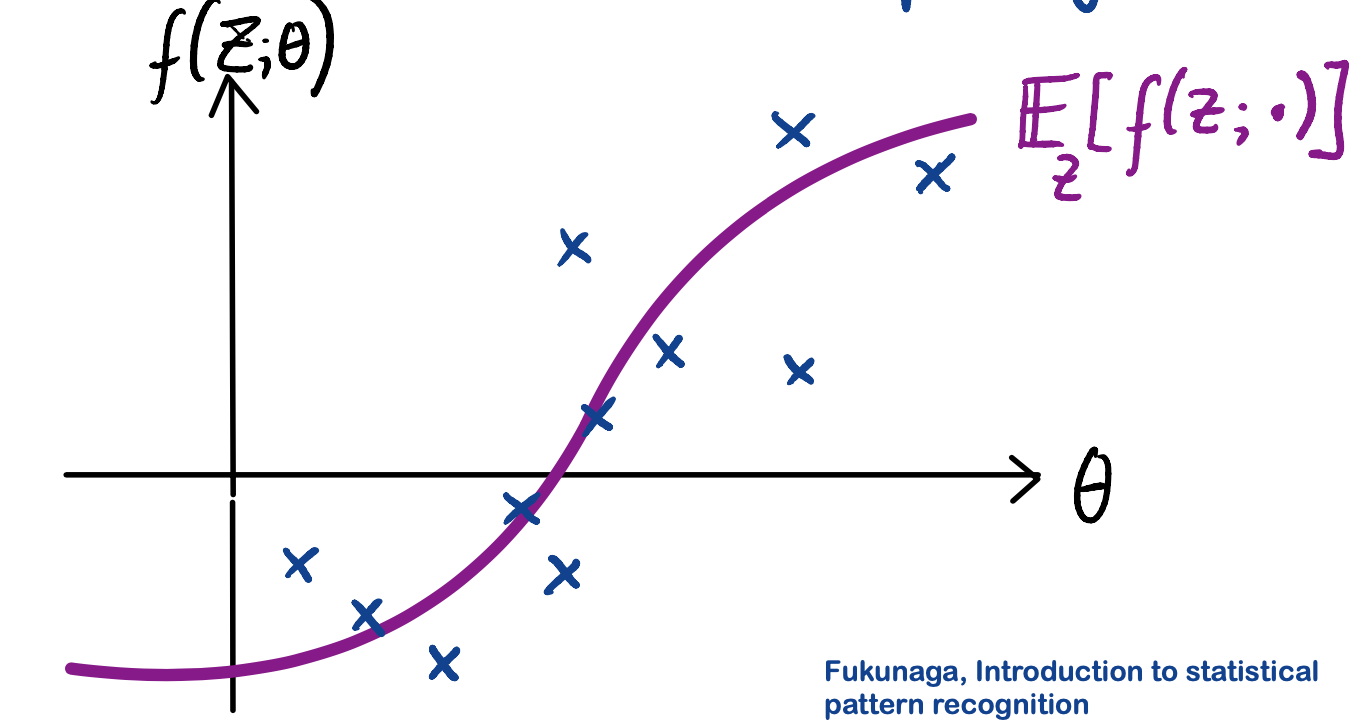
\includegraphics[width=\columnwidth]{images/10-robbin-monro}
\end{minipage}






	
	\subsection{Regularization in DNNs (Exercise 6.3) \\ Problems + Solutions}
\textbf{Dying ReLu Problem:} Once a value becomes negative, it will always output 0. Since the gradient for neg. values is 0 in ReLu, it will not become active again. 
\begin{itemize}
	\item[$\Rightarrow$]\textit{ELU or leaky ReLU activation function that has a non-zero gradient for arguments smaller than zero.}
	$$
	\mathit{ELU}_\alpha = 
		\begin{cases}
			\alpha(\exp(z) - 1) & z< 0 \\
			z 					& z\geq 0
		\end{cases}
	$$
	\textit{with hyperparamter $\alpha$}.
\end{itemize}



\textbf{Slow learning of a DNN with sigmoid function using Gradient Descent algorithm and large initialized weights:} ) The sigmoid function saturates quickly and hence, for large values of $z$ the gradient updates are very small, slowing down the learning process.
\textit{\begin{itemize}
	\item[$\Rightarrow$] Use random initialization weights 
	\item[$\Rightarrow$] Apply different activation function( such as ReLU or its variations), that is nonsaturating for positive values
\end{itemize}
}


\textbf{Applying dropout layers to avoid overfitting: } This will increase the training time, since parameter updates become noisy due to omitting units in each training iteration.  \\
Inference time is not influenced, since dropout is only applied during training

\subsection{Variational Autoencoders (Notes 11)}
\textit{Learn meaningful representations without supervision.
}\begin{center}
\textbf{Representation Learning: }
	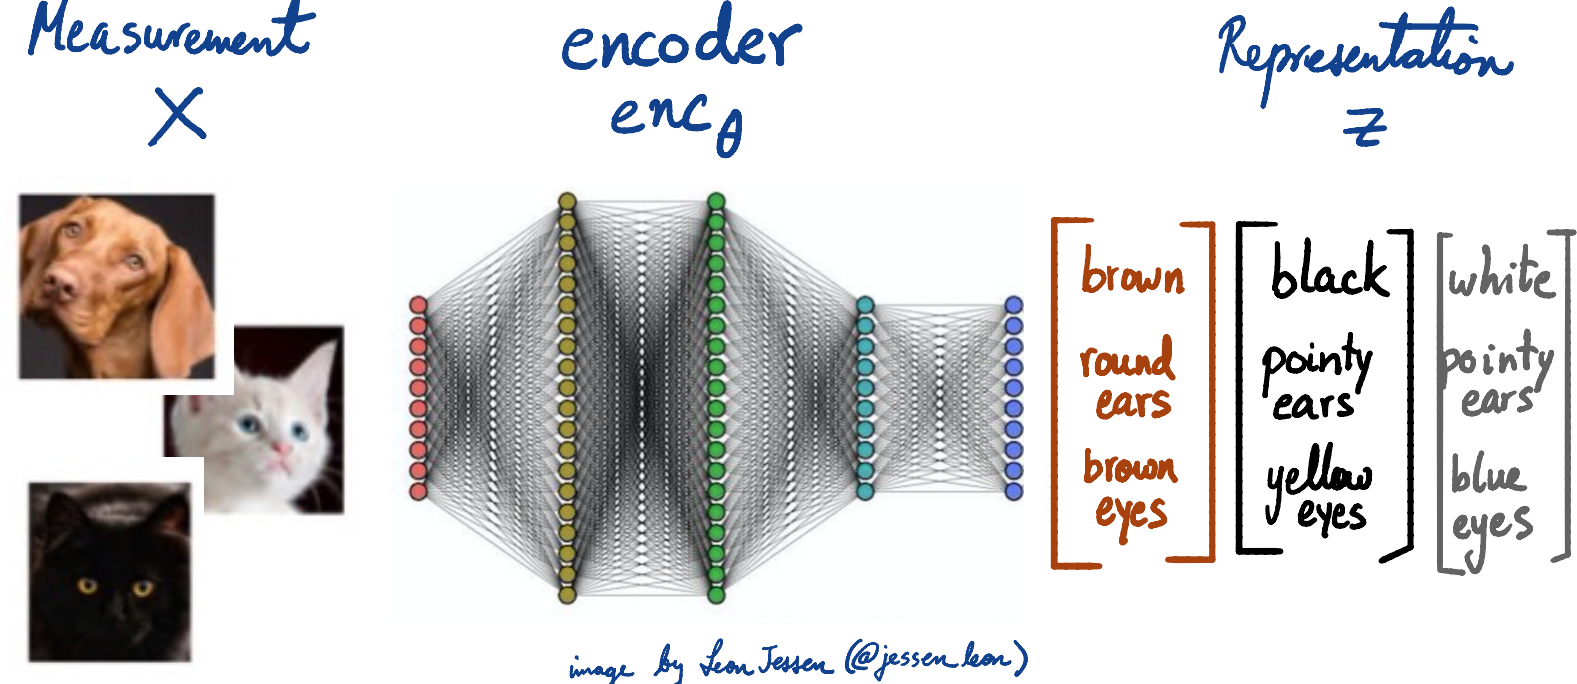
\includegraphics[width=0.8\columnwidth]{images/11-representation-learning}
\end{center}

\subsubsection{Objective}
Derive parametrized function $\enc_\theta$ that maps measurements in $\mathcal X$ to probability distributions over a representation space $\mathcal Z$
$$
	\enc_\theta: x \in \mathcal X \mapsto p_\theta(\cdot| x) \textit{ over } \mathcal Z 
$$


\textbf{Requirements for Autoencoder:}
\begin{itemize}
	\item Informative: Given representation, it should be easy to guess the measurement
	\item Disentangled: Every component in the representation is associated with a distinguished feature
	\item Robust: Noisy perturbations in the measurement should not substantially affect the representation and vice versa
\end{itemize}

\subsubsection{The info max principle (Linsker 1988)}
$Z = \enc_\theta(X)$ maximizes $I(X;Z)$

Information $(X;Z)$ is defined as
$$
	I(X;Z) = \E_{X,Z}\left[\log\left(\frac{p(X,Z)}{p(X)p(Z)} \right) \right]
$$
\begin{center}
	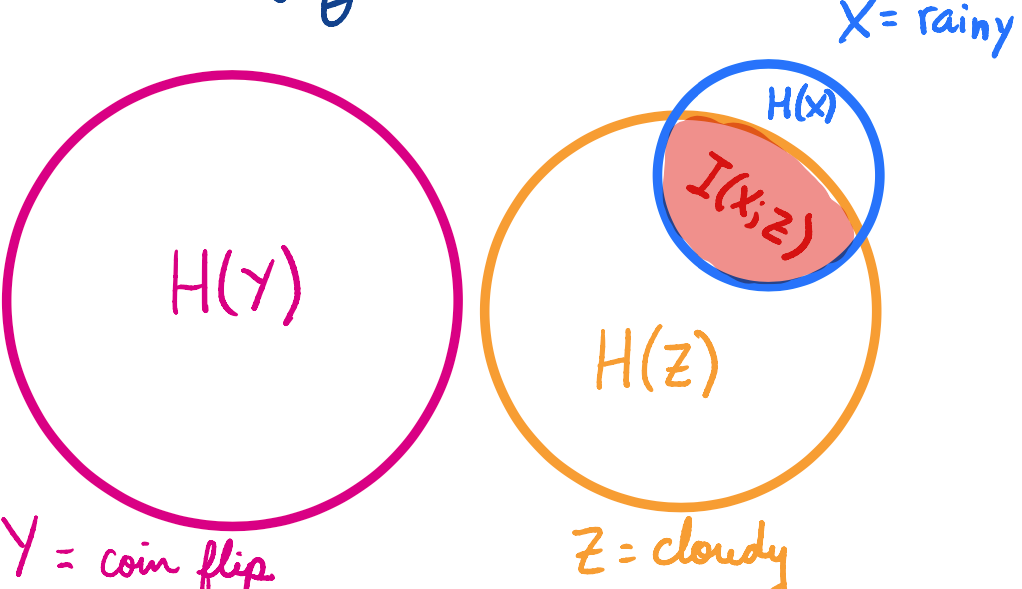
\includegraphics[width=0.5\columnwidth]{images/11-infomax-principle}
	$$
		H(x) = \E_x\left[-\log p(x)] \right]
	$$
\end{center}


\begin{minipage}{\columnwidth}
\textbf{Formalization}\\
Let $X$ and $Z$ be a measurement and a representation space. Let $F=\{\enc_\theta: \theta \in \Theta \}$ be a parametric family of functions with $\enc_\theta$ mapping $X$ to distributions over $Z$.

The encoder function $\enc_{\theta^*}$ is defined by 
$$
	\theta^* = \arg\max_\theta I(X; Z)
$$
where $Z$ is a random variable with distribution $\enc_\theta(X)$

This is informative, but not disentangled or robust. If $\enc_\theta$ is complex enough then $\enc_\theta$ maximizes $I(X;z)$ becoming an injective function from $X$ to $Z$.
	
\end{minipage}



\subsubsection{Variational Autoencoders (VAE)}
\textit{A VAE fits a generative probabilistic model to the dataset, where the representations are latent variables.}

\begin{minipage}{0.3\columnwidth}
	\begin{center}
		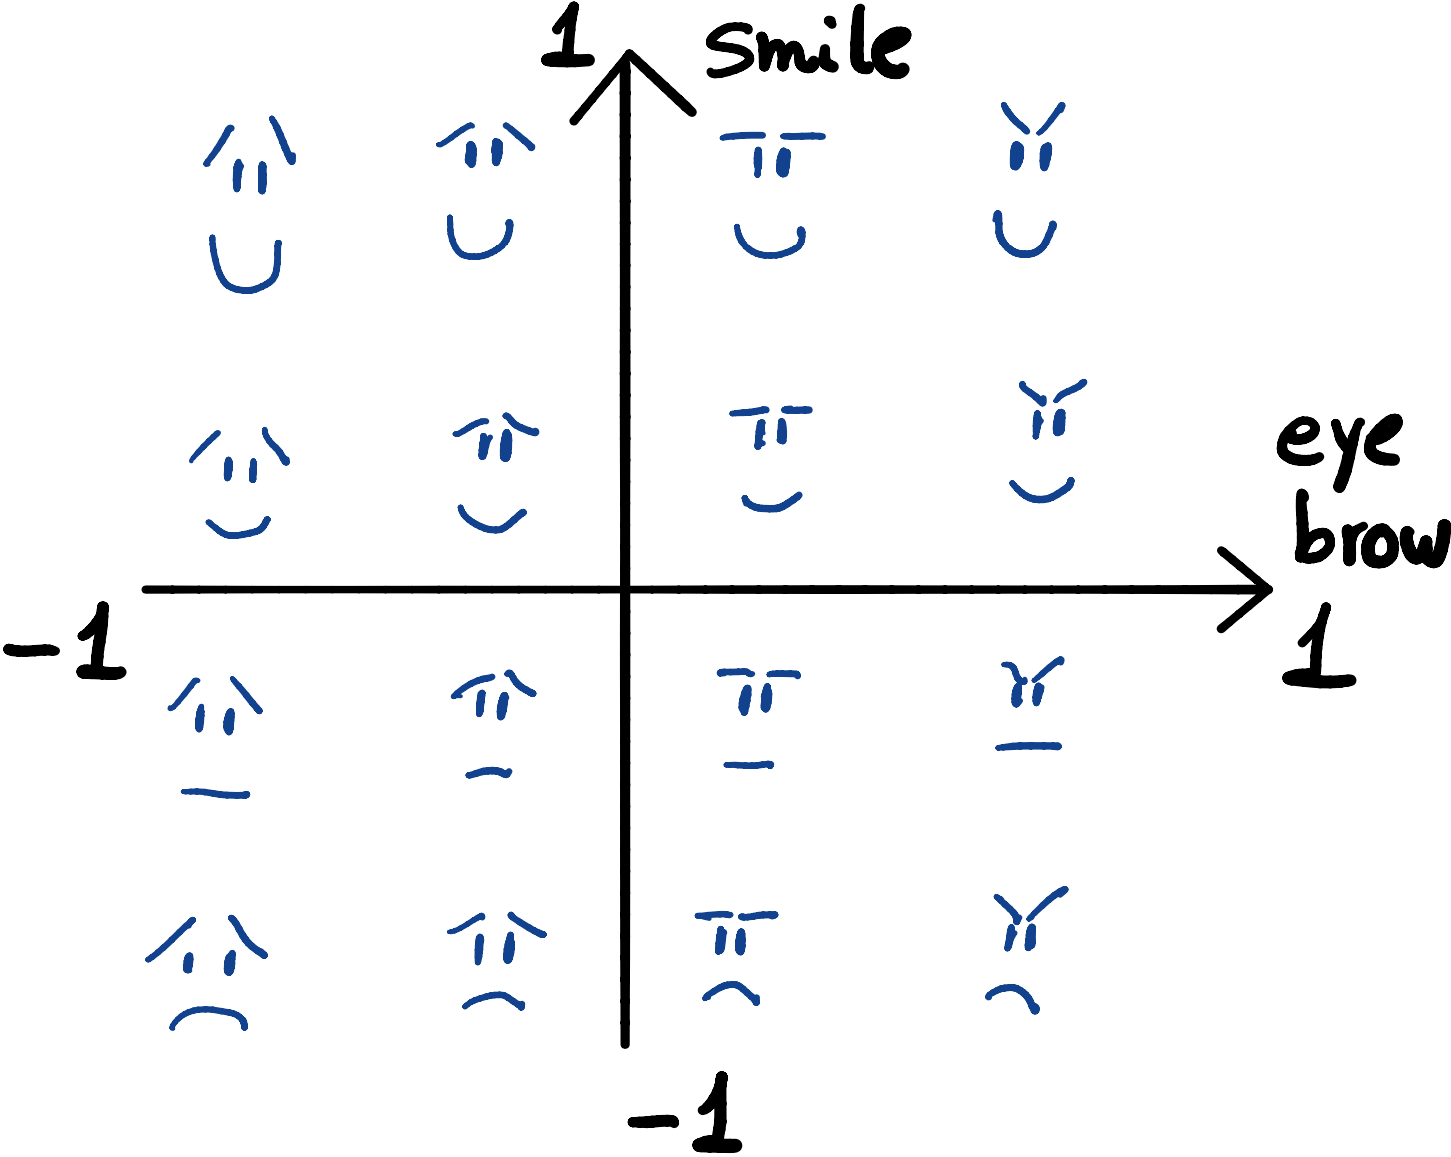
\includegraphics[width=\columnwidth]{images/11-autoencoders}
	\end{center}
\end{minipage}
\begin{minipage}{0.6\columnwidth}
\textbf{Smileys Example}
	\begin{itemize}
	\item Disentangled: $Z_0, Z_1$ along axes; in either direction only the smile OR the eye brows change
	\item Diagonal lines would be entangled.
\end{itemize}
\end{minipage}

\href{https://towardsdatascience.com/understanding-variational-autoencoders-vaes-f70510919f73}{Blogpost Link}

\textbf{Autoencoders: }
\begin{itemize}
	\item General Idea: Set an encoder and a decoder as neural networks and to learn the best encoding-decoding scheme using an iterative optimization process.
	\item At each iteration, compare encoded-decoded to initial data.
\end{itemize}



\textbf{Variational Autoencoders: }
\textit{Pick a family of distributions over the latent variables with its own variational parameters $q(z_{1:m}| \mathcal V)$. Then find the parameters that makes $q$ close to the desired posterior and use $q$ with the fitted parameters as a proxy for the posterior.} \href{https://www.cs.princeton.edu/courses/archive/fall11/cos597C/lectures/variational-inference-i.pdf}{(Princeton Advanced Methods in Probabilistic Modeling)}.

\begin{itemize}
	\item General Idea: autoencoder whose training is regularized to avoid overfitting and ensure that the latent space has good properties that enable generative process
	\item Autoencoders train encoder-decoder, but there is no way \textbf{generating new data}
	\item instead of encoding an input as a single point, encode it as a distribution over the latent space.
	\item In order to use an autoencoder for content generation, we have to make sure the distribution is regular (e.g. by using regularization terms).
\end{itemize}

\textbf{Variational Inference: } The process of finding an approximate posterior.
\begin{enumerate}
	\item Define prior and calculate likelihood (decoder)
	\item Find approximate posterior (encoder)
\end{enumerate}

\begin{highlight}{Variational Autoencoders}
\begin{enumerate}
	\item Define 
	\begin{itemize}
		\item $\{p_\theta'(z): \theta'\in \Theta'\}$ pram. family of priors
		\item $\{p_\theta(x|z): \theta\in \Theta\}$ pram. family of likelihoods
		\item $\{q_\phi(z): \phi\in \Phi'\}$ pram. f. of approx. posteriors
	\end{itemize}
	\item The variational auto encoder is trained by solving 
	$$
		\max_{\theta', \theta, \phi}\log p_{\theta', \theta, \phi}(x_1, ..., x_n), \{x_1, ..., x_n\} \textit{ training set}
	$$
	\item The representation $Z$ of a measurement $x$ is a random variable with pdf $q_\phi(z|x)$.\\ The measurement $X$ encoded by a representation $Z$ is a random variable with pdf $p_\theta(x|z)$
\end{enumerate}
\end{highlight}


\textbf{How to train a variational autoencoder? }
$$
	\arg\max_{\theta', \theta, \phi} \sumin \log p_{\theta', \theta}(x_i)
$$
{\footnotesize
\begin{align*}
	\log_{\theta', \theta}p(x_i) 	&= \E_{Z\sim q_\phi(\cdot| x_i)}\left[\log p_{\theta', \theta}(x_i)\right] \\
									&= \E_{Z\sim q_\phi(\cdot| x_i)}\left[\log \left(\frac{p_{\theta', \theta}(x_i, Z)}{p_{\theta'. \theta}(Z| x_i)}\frac{q_\phi(Z| x_i)}{q_\phi(Z| x_i)} \right)\right] \\
									&= \underbrace{\E_{Z\sim q_\phi(\cdot| x_i)}\left[\log \left(\frac{p_{\theta', \theta}(x_i, Z)}{q_\phi(Z| x_i)} \right)\right]}_{\mathit{elbo}_{\theta', \theta, \phi}(x_i)} \\
									&\quad\quad\quad  + \underbrace{E_{Z\sim q_\phi(\cdot| x_i)}\left[\log \left(\frac{q_\phi(Z| x_i)}{p_{\theta', \theta}(Z| x_i)} \right)\right] }_{\mathit{KL}\left(q_\phi(\cdot| x_i)\| p_{\theta', \theta}(\cdot| x_i)\right) \geq 0} \\
	\implies \log_{\theta', \theta}p(x_i) 
									&\geq \mathit{elbo}_{\theta', \theta, \phi}(x_i) \\
									&= \underbrace{\E_{Z\sim q_\phi(\cdot| x_i)}\left[\log \left(p_\theta(x_i| Z\right)\right]}_{\mathit{Infomax!}} \\
									&\quad\quad\quad  + \underbrace{E_{Z\sim q_\phi(\cdot| x_i)}\left[\log 
											\left(\frac{p_{\theta'}(Z)}{q_{\phi}(Z| x_i)} \right)\right] }_{\underbrace{\mathit{-KL}\left(q_\phi(\cdot| x_i)\| p_{\theta', \theta}(\cdot)\right) }_{\mathit{Regularization Term}}}  
\end{align*}
}
This is informative, disentangled and robust by the choice of $p_\theta(\cdot | Z)$ and $q_\phi(\cdot | x)$.
\subsubsection{Kullback-Leibler Divergence $\mathit{KL}$}
Used to measure the closeness of 2 distributions. Usually one of them is the approximation for the other. In our case: $q$ and $p$.
$$
	\mathit{KL}(q\|p) = \E_q\left[\log\frac{q(Z)}{p(Z|x)} \right]
$$
\subsubsection{The evidence lower bound $\mathit{elbo}$}
\textit{We can't minimize the KL divergence exactly. But we can minimize a function that is equal to it up to a constant: The $\mathit{elbo}$-function}

\textbf{The elbo is optimized using}
\begin{itemize}
	\item Gradient Descent
	\item Monte-Carlo Sampling
	\item Analytical Reparametrization tricks
\end{itemize}


\subsubsection{Denoising an Autoencoder}
Blank out parts of the input image during training to create a more robust encoder.

\subsubsection{Modeling Invariances}
If we want the autoencoder to be robust against rotations or scaling:
\begin{itemize}
	\item[$\Rightarrow$] Augmentation of training set
	\item[$\Rightarrow$] Special preprocessing of images
	\item[$\Rightarrow$] Implementation of invariances into multi-layer perceptrons (CNN) 
\end{itemize}

\subsection{Deep Generative Modeling}
We want to use generative modeling with DNN.


\subsubsection{Generative Adversarial Networks (GANs)}
\textit{Approach to generative modeling using deep learning methods (e.g. convolutional neural networks). In contrast to VAE, we do not model the density, but instead directly define a \textbf{sampler}.}\\
\textit{(Not covered in exam)}

\subsubsection{VAEs vs. GANs}
\begin{tabular}{ p{0.45\columnwidth} | p{0.45\columnwidth} }
		\textbf{VAE} & \textbf{GAN}\\\hline
  		\textbf{Pros: }
  		\begin{itemize}[leftmargin=*]
  			\item Principled approach
  			\item Allows inference of the encoder which might be useful for other tasks
  		\end{itemize}
  		& 
  		\textbf{Pros: }
  		\begin{itemize}[leftmargin=*]
  			\item Beautiful
  			\item State of the Art
  		\end{itemize}
  		\\\hline

  		\textbf{Cons: }
  		\begin{itemize}[leftmargin=*]
  			\item Maximizes the lower bound of the likelihood (quality is not as good, blurry)
  		\end{itemize}
  		&
  		\textbf{Cons: }
  		\begin{itemize}[leftmargin=*]
  			\item Tricky, unstable training
  			\item mode collapse
  			\item cannot solve inference queries as $p(x)$
  		\end{itemize} \\\hline
\end{tabular}


	\section{Clustering}
\textit{Given a training set, group the data into a few clusters. }

\textbf{Data Representation:}
\begin{itemize}
	\item Vector data: $n$ vecotrs in $\R^d$
	\item Histogram data:  $n$ histograms in $\R^d$
	\item Proximity data:  $n \times n$ pairwise proximity matrix. Much harder problem (structure hidden in $n^2$ pairwise relations

\end{itemize}
\subsection{$k$-means vs. EM}
\begin{tabular}{ p{0.45\columnwidth} | p{0.45\columnwidth} }
		\textbf{k-means} & \textbf{EM}\\\hline
		 \textbf{Objective: } minimize inter-cluster variance & \\\hline
		 Hard assignment & Soft assignment \\\hline	
  		works well for homog. clusters (assumes spherical clusters, with equal covariance matrices) & Can constrain algorithm to get different shapes of cov-matrices (not limited to spherical shapes)\\\hline
\end{tabular}

Neither of the algorithms can detect outliers! This would need a preprocessing step. In the presence of outliers, EM is more sensitive, since there are no constraints on the covariance matrix.

\subsection{$k$-means}
\subsubsection{$k$-means Problem}
\textit{Group data into $k$ groups.}

\begin{itemize}
	\item Given: $d$-dimensional sample vectors $\X$
	\item Assignment function
	\begin{equation*}
		\begin{gathered}
			c: \R^d \to \{1, ..., k\} \\
			\x \mapsto c(\x)
		\end{gathered}
	\end{equation*}
	\item Prototypes $\mu_c \in \mathcal Y \subset \R^d$
	\item \textbf{Problem: } find $c(.)$ and $\mathcal Y$ that minimize
	$$
		\mathcal R^{km}(c,\mathcal Y) = \sum_{x\in X}\norm{x - \mu_{c(x)}}^2
	$$
\end{itemize}

\subsubsection{$k$-means algorithm}

\begin{algorithm}[H]  
	\SetKwInOut{Input}{input}
	\SetKwInOut{Init}{init}

	\Input{$\mathcal X =\{\x_1, ..., \x_n\}$}
	\Init{$\mu_c =\x_c$ for $ 1\leq c\leq k$}

	\RepeatUntil{Changes of $c(\x), \mathcal Y$ vanish}{
		Keep prototypes $\mathcal Y$ fixed and assign sample vector $\x$ to neareast prototype 
		$$
			c(\x) \in \argmin_{c\in \{1, ..., k\}} \norm{\x-\mu_c}^2
		$$ \\
		Keep assignments $c(\x)$ fixed and estimate prototypes 
		$$
			\mu_\alpha = \frac{1}{n_\alpha} \sum_{\x:c(\x)=\alpha} \x, \text{ with $n_\alpha = \text{\#}\{\x:c(\x) = \alpha\}$}
		$$
  	}
  	\Return{$c(\x), \forall \x\in \mathcal X$ and the prototypes $\mathcal Y$}
  \caption{$k$-means algorithm}
\end{algorithm}

\subsection{Mixture Model}
Data are assumed to be distributed according to a density. When multiple sources are considered as potential causes for an observed example, this is a mixture model with the density for a feature vector $\x$:
$$
	p(\x|\pi_1, ..., \pi_k, \theta_1, ..., \theta_k) = \sum_{c\leq k} \pi_c p(\x|\theta_c)
$$
the mixture weight $\pi_c$ is the prior probability that a sample is generated by the mixture component $c$ with parameters $\theta_c$ (i.e. $\pi_c = p(c(\x) = c, \theta_c$).

\subsubsection{Gaussian Mixtures}
\textit{$\x$ was drawn from one of $k$ gaussians, depending on the class .}
\begin{itemize}
	\item Parameters $\theta = (\mu, \Sigma)$
	$$
		p(\x|\mu,\Sigma) = \frac{1}{\sqrt{2\pi}^d}\frac{1}{\sqrt{\|\Sigma|}}\exp\left(-\frac{1}{2}(\x - \mu)^T\Sigma^{-1}(\x - \mu) \right)
	$$
	\item Estimate $\hat\theta$ that maximizes the likelihood of sample feature vectors $\mathcal X = \{\x_1, ..., \x_n\}$
	$$
			p(\mathcal X|\pi_1, ..., \pi_k, \theta_1, ..., \theta_k) = \prod_{x\in \mathcal X}\sum_{c\leq k} \pi_c p(\x|\theta_c)
	$$
	\item Log-Likelihood 
	$$
	L(\mathcal X|\pi_1, ..., \pi_k, \theta_1, ..., \theta_k) = \sum_{x\in \mathcal X}\log \sum_{c\leq k}\pi_cp(\x|\theta_c)
	$$
\end{itemize}
Direct optimization of the log-likelihood is intractable due to sum within the logarithm (i.e. there is \textbf{no closed form solution}). 

EM Mixture models solve this by introducing latent indicator variables for mode assignments and maximizing the joint likelihood of the observable and latent variables.

\subsection{Expectation - Maximization algorithm}

\textbf{Principle: }
\begin{enumerate}
	\item Calculate $Q(\theta; \theta^{(j)}) = \E_{\mathcal X_L}\left[L(\mathcal X, \mathcal X_L|\theta) \middle\vert \mathcal X, \theta^{(j)}\right]$ \\
		\textit{Function of parameters given the parameters in the step before.}
	\item Estimate new parameters by maximizing the log-likelihood of $Q$: 
	$$\theta^{(j+1)}\in \argmax_{\theta}Q(\theta; \theta^{(j)})$$
	\item Repeat until convergence
\end{enumerate}
\textit{\textbf{Derivations: } (Full derivations on p. 11 - 16, Lecture 12 - clustering)}
$$
	M_{\x c} = 
	\begin{cases}
		1 &\textit{Mode $c$ has generated vector $\x$} \\
		0 &\textit{Mode $c$ has not generated vector $\x$}
	\end{cases}
$$

This gives
\begin{align*}
	P(\mathcal X, M|\theta) &= \prod_{x\in\mathcal X}\prod_{c=1}^k(\pi_c P(\x|\theta_c))^{M_{\x c}}\\
	L(\mathcal X, M|\theta) &= \log P(\mathcal X, M|\theta) =\sum_{x\in\mathcal X}\sum_{c=1}^k M_{\x c}(\pi_c P(\x|\theta_c))
\end{align*}

We define
$
	\gamma_{\x c} := \E_M\left[M_{\x c}\middle \vert \mathcal X, \theta^{(j)}\right]
$



\begin{algorithm}[H]  
	
	\RepeatUntil{Changes are small enough}{
		\textbf{E-Step: For all $c$}
		$$
			\gamma_{\x c} = \frac{P(\x|c, \theta^{(j)}P(c|\theta^{(j)})}{P(\x|\theta^{(j)})}
		$$	\\
		\textbf{M-Step: For all $c$}
		\begin{align*}
			\mu_c^{(j+1)} &= \frac{\sum_{\x\in \mathcal X}\gamma_{\x c}\x}{\sum_{\x\in \mathcal X}\gamma_{\x c}} \\
			(\sigma_c^2)^{(j+1)} &= \frac{\sum_{\x\in \mathcal X}\gamma_{\x c}(\x-\mu_c)^2}{\sum_{\x\in \mathcal X}\gamma_{\x c}} \\
			\pi_c^{(j+1)} &= \frac{1}{|\mathcal X|}\sum_{\x\in \mathcal X}\gamma_{\x c}
		\end{align*}	
  	}
  \caption{Expectation-Maximization Algorithm}
\end{algorithm}

\subsection{Problems with Mixtures of Gaussians}
\begin{itemize}
	\item Computation time: Time to estimate the model parameters may be large
	\item Number of free parameters: Scales with $O(d^2)$ ($d$ data dimension)
	\begin{itemize}
		\item[$\Rightarrow$] Param. estimation problematic if dimension of features space is high and number of samples is slow
		\item[$\Rightarrow$] \textbf{Solution: } Use only hard assignments $c(x) \in \{1, ..., k\}$ as in $k$-means clustering.
	\end{itemize}	
\end{itemize}


	\section{Non-Parametric Bayesian Methods}
\begin{itemize}
	\item \textbf{Beta Distribution}
	$$
		\mathit{Beta}(x|a,b) = \frac{1}{B(a,b)}\cdot x^{a-1}(1-x)^{b-1}, x\in [0,1]; a,b > 0
	$$
	where 
	\begin{equation*}
		\begin{gathered}
			B(a,b)  =\frac{\Gamma(a)\Gamma(b)}{\Gamma(a + b)}\\
			\Gamma(a) = \int_0^\infty e^{-x}x^{a-1}dx
		\end{gathered}	
	\end{equation*}
	\textit{Probability of a Bernoulli process after observing $a-1$ successes and $b-1$ failures}
	\item \textbf{Dirichlet Distribution:} Multivariate generalization of the beta distribution.\\
	\textit{Given $\x = x_1, ..., x_n, \alpha = \alpha_1, ..., \alpha_n$ where $x_i\in [0,1], \alpha_i > 0$}
	$$
		\mathit{Dir}(\x|\alpha) = \frac{1}{B(\alpha)}\cdot \prod_{k=1}^n x_k^{\alpha_k-1}
	$$
	\textit{where $B(\alpha)$ is the multivariate generalization of the beta function: }
	$$
		B(\alpha) = \frac{\prod_{k=1}^n \Gamma(\alpha_k)}{\Gamma(\sum_{k = 1}^n \alpha_k)}
	$$
	\begin{center}
		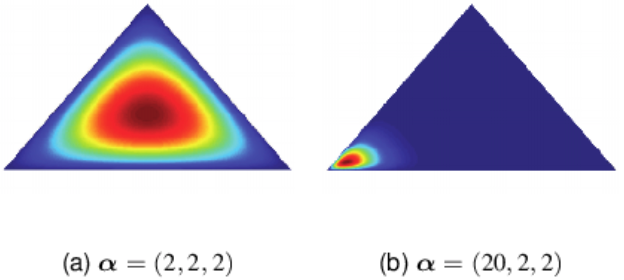
\includegraphics[width=0.8\columnwidth]{images/12b-dirichlet}
	\end{center}
	
\end{itemize}
\subsection{Finite and infinite mixtures}
\subsubsection{Finite Gaussian Mixture Model: } Fixed, finite number of clusters $K$
	\begin{itemize}
		\item Center of cluisters $\mu_k\sim \mathcal N(\mu_0, \sigma_0)$
		\item Prob. of the clusters (parameters) $\rho_{1...K}\sim \mathit{Dir}(\alpha_{1...K})$
		\item Assignments to clusters $z_i\sim \mathit{Categorical}(\rho_{1...K})$
		\item Coordinates of data points $x_i \sim \mathcal N(\mu_{z_i}, \sigma_{z_i})$
	\end{itemize} 
\subsubsection{Selecting $K$: }
\textbf{Issues: }
\begin{itemize}
	\item There might be multiple possible ways to cluster data (hence multiple $K$ that would fit)
\end{itemize}

\textbf{Adaptation: }
\begin{itemize}
	\item Number of clusters might be unknown in advance (movie genres, topics of documents, image segmentation, streaming data, ...)
	\item Naive solution: Select $K$, cluster with EM, evaluate the result and iterate
\end{itemize}

\textbf{What if we just select a large enough $K$? }

\begin{minipage}{\columnwidth}
	\begin{center}
		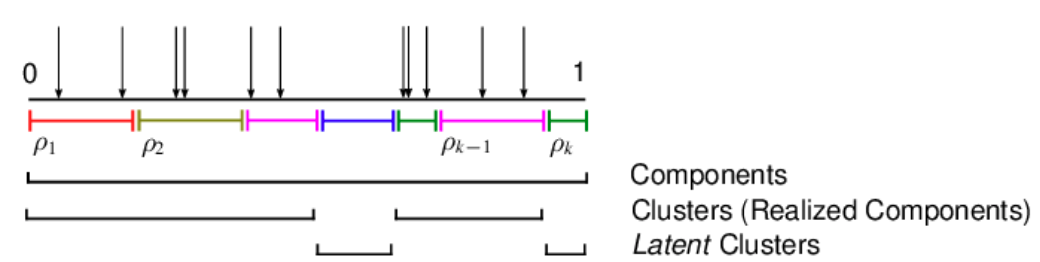
\includegraphics[width=\columnwidth]{images/12b-latent-clusters}
	\end{center}
	\textit{\textbf{Latent clusters: }For a finite number of drawings $N$, we do not have to realize all $K$ clusters. All components will be realized with probability $1$, but only when $N\to\infty$}
\end{minipage}

\begin{itemize}
	\item Select a large $K$, only realize some of them and get more when needed
	\item This only solves the problem partially: How large should this $K$ be? Our belief in $K$ could change as we observe more data-points. We still have issues with streaming/growing data.
	\item \textbf{Solution: Select $k=\infty$}
\end{itemize}

\subsubsection{Infinite mixture models (Selecting $K=\infty$)}
\begin{itemize}
	\item With $K=\infty$, we have nonparametric Bayesian methods (nonparametric means infinitely many parameters) $\to$ we can keep drawing new parameters
	\item Cannot draw infinite points from $\mathit{Dir}$
\end{itemize}




\subsection{Dirichlet Process (DP) and stick breaking}
We can \textbf{sample from a DP using either Stick-Breaking or the Chinese Restaurant Process}

\subsubsection{Dirichlet Proces}
$\DP(\alpha, H)$ is a distribution over probability distributions on a space $\Theta$.
\begin{itemize}
	\item $\alpha\in\R_{>0}$ is a concentration parameter
	\item $H$ is the base measure on $\Theta$ (the space we want to draw parameters from)
	\item A Sample $G\sim\DP(\alpha, H)$ is a function $G:\Theta\to\R_{\geq 0}$ s.t. $\int_\Theta G(\theta)d\theta=1$
\end{itemize}

\begin{minipage}{\columnwidth}
$\DP(\alpha H)$ is characterized by the following property: \textit{For every partition $(T_1, .., T_k)$ of $\Theta$ and $G\sim \DP(\alpha, H)$ we have (for each tuple drawn from multivariate Dirichlet distribution): }

$$
	(G(T_1), ..., G(T_K))\sim \Dir(\alpha H(T_1), ..., \alpha H(T_k))
$$
\end{minipage}

\subsubsection{Stick-Breaking Process}
\textbf{Observation: } sampling $(\rho_1, ..., \rho_K) \sim \Dir(\alpha_1, ..., \alpha_K)$ is equivalent to sampling $\rho_1 \sim \Beta(\alpha_1, ..., \alpha_K)$ and $(\rho_2, ..., \rho_K) \sim \Dir(\alpha_2, ..., \alpha_K)$

\begin{center}
	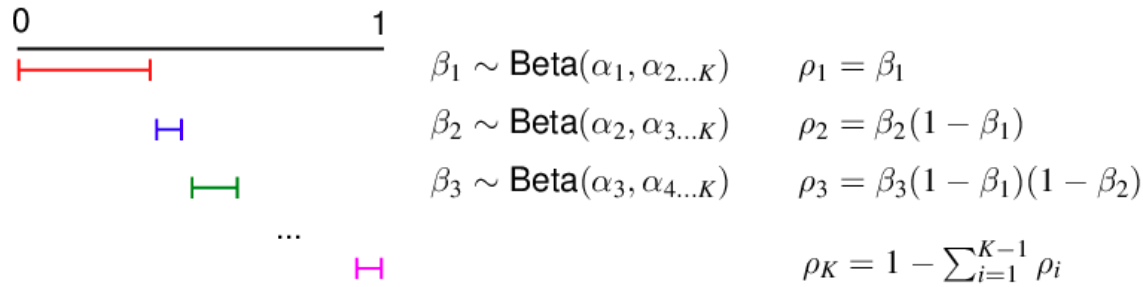
\includegraphics[width = 0.8\columnwidth]{images/12b-stick-breaking-1}
\end{center}
We can keep doing this, but only if $\alpha = (\alpha_1, ..., \alpha_K)$ has finite length $K$.

\textbf{Solution: } fix $\alpha$ s.t. $\beta_i\sim \Beta(1, \alpha) \forall i$
\begin{center}
	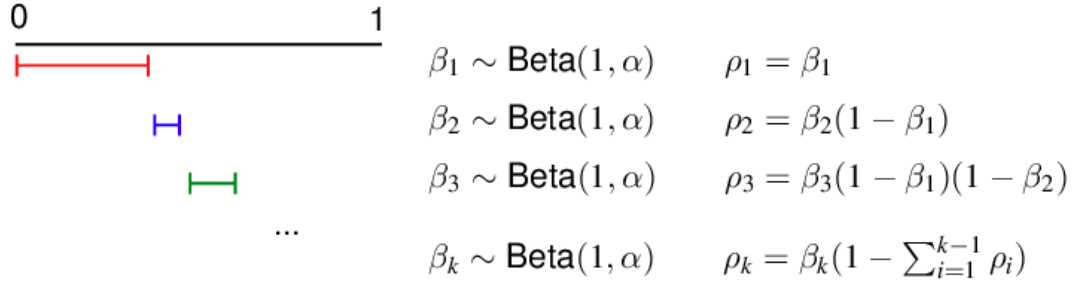
\includegraphics[width =  0.8\columnwidth]{images/12b-stick-breaking-2}
\end{center}

This is called the GEM (Griffiths-Engen-McCloskey) distribution: 
$$
	\rho\sim \GEM (\alpha), \rho.= \{p_k\}_{k = 1}^\infty	
$$

\textbf{Stick-Breaking Construction of the Dirichlet Process: }\\
If $\rho\sim \GEM(\alpha)$ and $\theta_k\sim H$ for $k = 1, 2, ...$, then 
$$
	G(\theta) = \sum_{k=1}^\infty\rho_k\delta_{\theta_k}(\theta)
$$
is a sample from $DP(\alpha, H).$

If we repeatedly sample $\theta^{(1)}, \theta^{(2)}, ...$ from $G\sim \DP(\alpha, H)$, then we have $\theta^{(i)} = \theta_{k_i}$ for some $k_i$.
\begin{itemize}
	\item Sometimes we get a new value $(k_i\neq k_j \forall i<j)$
	\item Sometimes we get a repetition$(k_i =  k_j \text{ for some } i<j)$
	\item Think of $\theta^{(i)}, \theta^{(j)}$ with $k_i = k_j$ as points belonging to the \textbf{same cluster}.
\end{itemize} 

\subsubsection{Chinese Restaurant Process}
\textbf{Technique to draw samples from a Dirichlet Process: }
\begin{itemize}
	\item Join an existing table with probability $\propto$ the number of people already sitting there
	\item Start a new table with probability $\propto \alpha$
\end{itemize}
$$
	P(\textit{customer $n+1$ joins table $\tau$}|\mathcal P) = 
		\begin{cases}
			\frac{|\tau|}{\alpha + n} & \textit{if $\tau \in \mathcal P$} \\
			\frac{\alpha}{\alpha + n} & \textit{Otherwise}
		\end{cases}
$$
\begin{itemize}
	\item $\alpha$ controls the number of new tables ($\alpha$ large: new table likely), 
	\item $|\tau|$ is the number of people on table $\tau$
	\item $\mathcal P$ is a table assignment (partition over the integers)
\end{itemize}


\textbf{Expected number of tables (i.e. clusters) created: }
$$
	\E[\textit{created tables}] = \sumi N\frac{\alpha}{\alpha + i} \sim O(\alpha\log(N)) ]
$$
\textit{"Rich-get-Richer"-effect (preferential attachment): Already popular clusters attract new datapoints}
\subsubsection{Exchangeability}
\textbf{Definition: } Let $(X_1, X_2, ...)$ a sequence of random variables. The sequence is exchangeable when, for every permutation $\pi$ of $\N$. The random vectors
$$
	(X_1, X_2, ...) \quad \textit{ and } \quad (X_{\pi(1)}, X_{\pi(2)}, ...)
$$
have the same distribution.

\textbf{De Finetti's Theorem: } Let $(X_1, X_2, ...)$ be an infinitely exchangeable sequence (one that can be represented by conditionally independent random variables) of random variables. Then $\forall n$
$$
	p(X_1, ..., X_n) = \int \left(\prod_{i = 1}^n p(x_i|G)\right) dP(G)
$$
for some random variable $G$


\textbf{P\'{o}lya Urn}
\begin{itemize}
	\item Urn with colored balls
	\item Draw balls from the urn at random. After drawing a ball, put it back in the urn together with a new ball of the same color
\end{itemize}

\textbf{Hoppe Urn}: P\'{o}lya Urn with special black ball
\begin{itemize}
	\item Urn with colored balls
	\item Draw balls from the urn at random. After drawing 
	\begin{itemize}
		\item If non-black ball: put it back in the urn together with a new ball of the same color
		\item If black ball: put it back in the urn with a new ball of the same color
	\end{itemize}
\end{itemize}

\begin{highlight}{Exchangeability Results}
\begin{itemize}
	\item CRP is identical to the hoppe earn process (we just need to add colors to the tables)
	\item Hoppe Urn and CRP are exchangeable: Can apply \textbf{De Finetti's theorem}
	\item DP is the rancom variable $G$ in De Finetti's theorem for Hoppe urn / CPR
	\item If the prior of $G$ is the DP, then CRP is how we assign points to clusters when we integrate out $G$.
\end{itemize}
\end{highlight}
\subsection{The DP Mixture Model}
$\Theta$ is a set that parametrizes a set of probability distributions, $H$ fixed base measure on $\Theta$. Example:
\begin{itemize}
	\item $\Theta = \R$ with $\mu\in \Theta$ corresponding to $\mathcal N(\mu, \sigma)$ for some fixed $\sigma > 0$
	\item $H = \mathcal N(\mu_0, \sigma_0)$ for some $\mu_0\in \R, \sigma_0\in \R$
\end{itemize}

Based on that we define the \textbf{DP Mixture Model} (a generative model):
\begin{itemize}
	\item Probabilities of clusters ("mixture weights"): $\rho = (\rho_1, \rho_2, ...)\sim\GEM(\alpha)$
	\item Center of clusters $\mu_k\sim \mathcal N(\mu_0, \sigma_0)$
	\item Assignments to clusters $z_i\sim \mathit{Categorical}(\rho)$
	\item Coordinates of data points $x_i \sim \mathcal N(\mu_{z_i}, \sigma)$
\end{itemize}

\subsection{Gibbs sampling}
Useful way of simulating from distributions that are difficult to simulate from directly.

Technique to fit the DPMM (EM considered difficult for nonparametric distributions) by sampling each variable in turn (conditioned on the values of all other variables in the distribution). \textbf{Requires exchangeability}.
\subsubsection{Fitting}
Leverage exchangeability: Any point can be considered "last arrived". Change the assignment of te element without influencing other assignments.
\begin{itemize}
	\item \textbf{Prior}: Probabilities of table assignments w.r.t people seating (cluster size)
	\item \textbf{Posterior}: Probability of the point given the cluster centers
\end{itemize}

\subsubsection{Gibbs Sampling for Fitting}
\begin{minipage}{\columnwidth}
\textbf{Probability Distribution: Collapsed Gibbs sampling formulation}
\begin{align*}
	&p(z_i=k|\z_{-i},\x,\alpha,\mu) \\	
		&\propto p(z_i=k|\z_{-i},\alpha,\cancel{\mu})p(\x|z_i=k,\z_{-i},\cancel\alpha,\mu) \\
		&\propto p(z_i=k|\z_{-i},\alpha)p(x_i|\x_{-i},z_i=k, \z_{-i},\mu)p(\x_{-i}|\z_{-i}, \mu) \\
		&\propto 	\underbrace{p(z_i=k|\z_{-i},\alpha)}_{\textit{Prior}}
					\underbrace{p(x_i|\x_{-i},z_i=k, \z_{-i},\mu)}_{\textit{Likelihood}}
\end{align*}
where $\z_{i}$ and  $\x_{i}$ are the assignments and points excluding the considered point $i$.
\end{minipage}

\textbf{Prior: }
$$
	p(z_i=k|\z_{-i},\alpha) = 
		\begin{cases}
			\frac{N_{k, -i}}{\alpha + N - 1} 	& \textit{For existing $k$} \\
			\frac{\alpha}{\alpha + N - 1} 		& \textit{otherwise} 
		\end{cases}
$$
where $N_{k, -i}$ is the number of elements sitting at table $k$ excluding $i$ $(|\tau\backslash i|)$

\textbf{Posterior: } Observe that if $z_i = k$ we don't need to consider points in $\x$ that are not in $k$. \\
Let $\x_{-i, c} = \{x_j:z_j=c, j\neq i\}$ the data assignment to cluster $c$, then

\begin{multline*}
	p(x_i|\x_{-i},z_i=k, \z_{-i},\mu) = \\
		\begin{cases}
			p(x_i| \x_{-i, k}, \mu) = \frac{p(x_i, \x_{-i, k}|\mu)}{p(\x_{-i, k}|\mu)} & \textit{for existing $k$} \\
			p(x_i|\mu) & \textit{otherwise}
		\end{cases}
\end{multline*}

\subsubsection{Final Collapsed Gibbs sampler: }
\begin{multline*}
	p(z_i=k|\z_{-i},\x,\alpha,\mu) = \textit{Prior} \times \textit{Likelihood} \\
	= \begin{cases}
			\frac{N_{k, -i}}{\alpha + N - 1} p(x_i| \x_{-i, k}, \mu)	& \textit{For existing $k$} \\
			\frac{\alpha}{\alpha + N - 1} p(x_i|\mu)		& \textit{otherwise} 
		\end{cases}
\end{multline*}
	
\begin{algorithm}[H]  
	\For{$i = 1$ to $N$ in random order}{
		Remove $x_i$'s sufficient statistics from old cluster $z_i$ \\
		\For{$k = 1$ to $K$}{
			Compute $p_k(x_i) = p_k(x_i|\x_{-i, k})$ \\
			Set $N_{k, -i} = |\x{-i, k}|$	\\
			Compute $p(z_i=k|\z_{-i},\x) = \frac{N_{k, -i}}{\alpha + N-1}p_k(x_i)$
		}
		Compute $p_*(x_i) = p(x_i|\mu)$ 		\textit{(new cluster)}\\
		Compute $p(z_i=*|\z_{-i}, \x)$ \\
		Normalize $p(z_i|\cdot)$ \\
		Sample $z_i\sim p(z_i|\cdot)$\\
		Add $x_i$'s sufficient statistics to new cluster $z_i$ \\
		If any cluster is empty, rmeove it and decrease $K$\\
	}
	\caption{Collapsed Gibbs sampler for DP mixtures}
\end{algorithm}

\subsubsection{Latent Dirichlet Allocation}
\begin{itemize}
	\item Popular nonparametric Bayesian method
	\item Extension of the model we just defined
	\item \textbf{support multivariate distributions} (e.g. topic modeling on documents, each document belongs to more than one topic; mixture over topics $\to$ multivariate)
\end{itemize}

Given $K$ topics and $V$ words in the vocabulary, for $M$ documents with $N$ words each:\\

\begin{minipage}{0.5\columnwidth}
Distribution of topics in doc. $d$: 
$$
	\theta_d\sim\Dir(\alpha)
$$

Topic that word $w$ in $d$ belongs to:
$$
	z_{d,w} \sim \mathit{Categorical}(\theta_d)
$$

Distribution of words in topic $k$:
$$
	\varphi_k \sim \Dir(\beta)
$$

word $w$ in document $d$: 
$$
	w_{d,w}\sim \mathit{Categorical}(\varphi_{z_{d,w}})
$$
\end{minipage}
\begin{minipage}{0.4\columnwidth}
	\begin{center}
		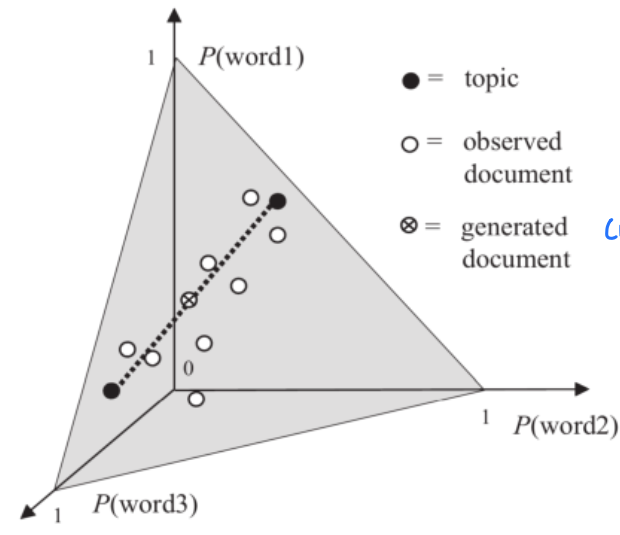
\includegraphics[width=\columnwidth]{images/12b-lda}
	\end{center}
	$\alpha$ controls prior weights of topics in documents, $\beta$ controls prior weights of words in topic
\end{minipage}




	\section{Probably Approximately Correct (PAC) Learning}
Machines can't compute everything. There are undecidable problems (Turning's halting problem, Post's correspondence problem). \\
Formal logic can't prove everything (G\"{o}del's incompleteness theorem: There are infinitely many truths about arithmetic that cannot be proven formally)
\begin{itemize}
	\item \textbf{Statistical Learning Theory: } Framework for ML aiming at learning \textbf{functions from data}
	\item \textbf{PCA learning: } subfield of ML concerned with the question of \textit{what is learnable and how much can we learn something by empirically minimizing a cost function}.
\end{itemize}

\begin{minipage}{\columnwidth}
\textbf{The learning problem:}
\begin{center}
	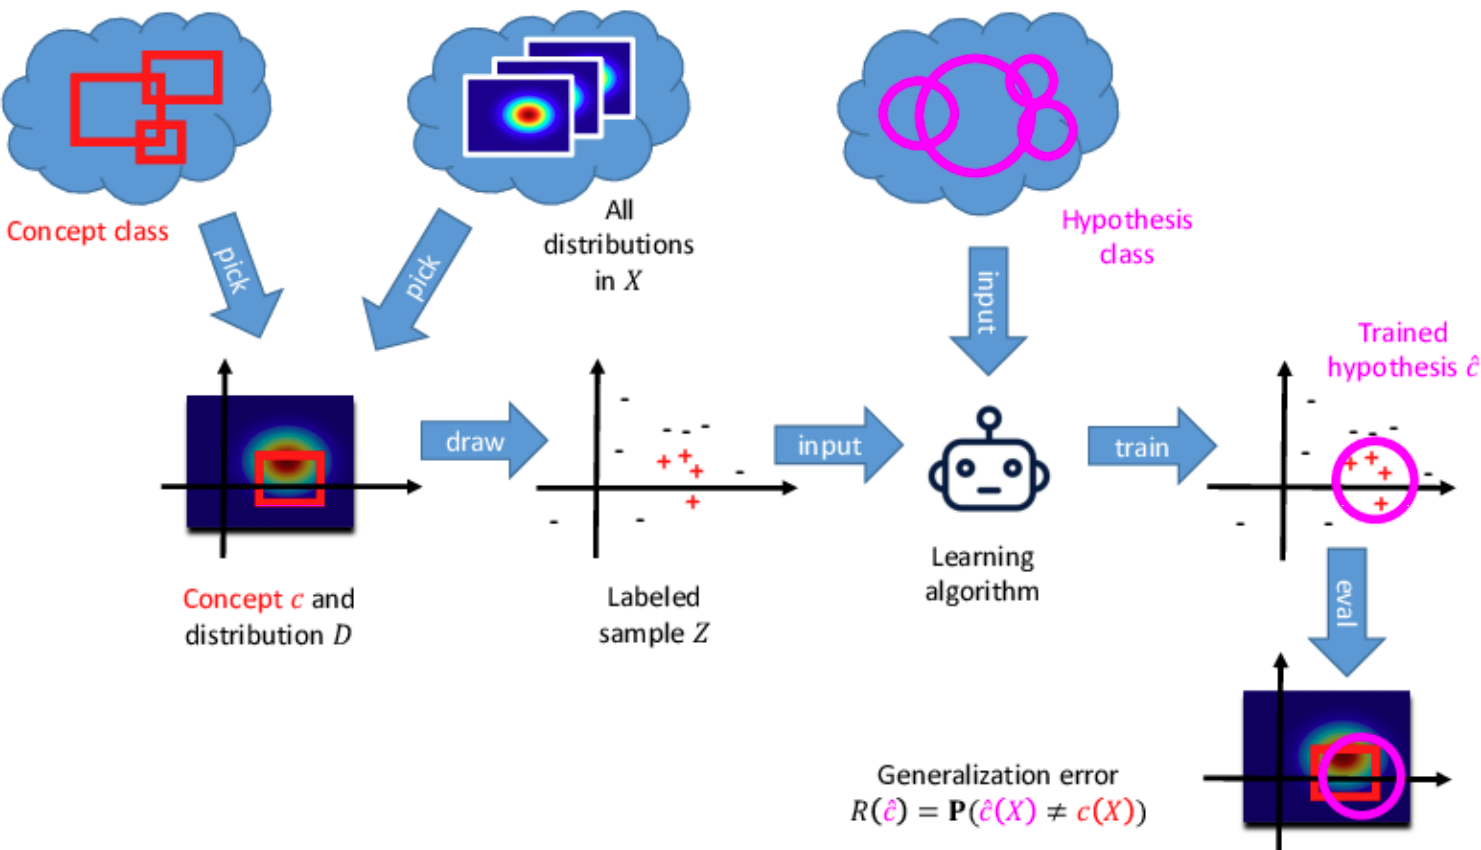
\includegraphics[width=\columnwidth]{images/13-learning-problem}
\end{center}
\end{minipage}
The generalization error measures the distance between the concept $c$ and the trained hypothesis $\hat c$.
\begin{itemize}
	\item The generalization error is not computable by the learner: \\ $\mathcal R(\hat c) := \P(\hat c(X) \neq c(X))$
	\item Empirical error is computable by the learner: \\
	$ \hat{\mathcal R}_n(\hat c) := \sumin \mathbf 1_{\hat c(x_i)\neq c(x_i)}$ \\
	It can be shown that $\E_{X, X_1, ..., X_N}\left[\hat{\mathcal R}_n(\hat c(X))\right] = \mathcal R(\hat c)$
\end{itemize}
\subsection{Notions from statistical learning theory}
\begin{itemize}
	\item \textbf{Instance space $\mathcal X$} Seit of instances or objects in the learner's world
	\item \textbf{Concept: } subset $c$ of $\mathcal X$ (function $c:\mathcal X\to \{0,1\}$ for binary classification).
	\item \textbf{Concept Class: } Set of concepts we wish to learn
	\item \textbf{Hypothesis class: } Other set of concepts that we use to learn a target concept from the concept class.
	\item No additional prior knowledge on $\mathcal X$ is available. This differs from Bayesian approaches.
\end{itemize}



\subsection{The PAC Learning Model}
\begin{itemize}
	\item A concept class $C$ is \textbf{PAC learnable} from a hypothesis class $\mathcal H$ if there is an algorithm that can lern every concept in $\mathcal C$.
	\item If the algorithm runs polynomial time to $1/\epsilon$ and $1/\delta$, we say that $\mathcal C$ is \textbf{efficiently PAC learnable}. ($\epsilon$ error parameter, $\delta$ confidence value)
\end{itemize}






\subsection{Rectangle Learning}
Axis-Aligned rectangles are PAC learnable.
\begin{itemize}
	\item $\mathcal C$ concept of all axis-aligned rectangles. \\
	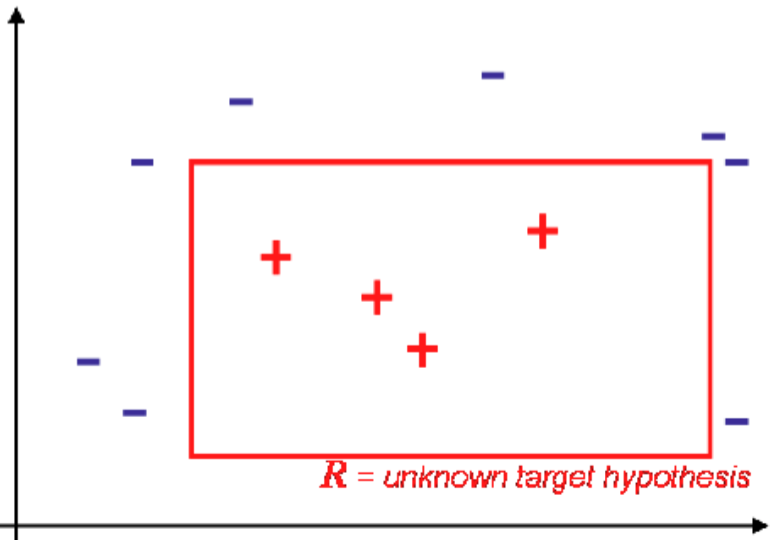
\includegraphics[width = 0.6\columnwidth]{images/13-rectangle-learning}
	\item We show $\mathcal C$ can be learned from $\mathcal H = \mathcal C$
	\item Consider $\mathcal A$ that outputs smalles rectangle $\hat R$ containing all positively labeled points. \textbf{We show that $\mathcal A$ can learn any concept $R\in \mathcal C$
}\end{itemize}

\textbf{How do we prove that $\mathcal A$ learns rectangles?}\\
\begin{itemize}
	\item Define event $\RIG$ \textit{($\hat{\mathcal R}$ is good enough)}, such that
	$$
		\P(\mathcal R(\hat R)\leq \epsilon) \geq \P(\RIG)\geq 1 - 4\exp\left(-\frac{n\epsilon}{4}\right)
	$$
	\item Observe we just need to ensure that $1 - 4\exp\left(-\frac{n\epsilon}{4}\right)\geq 1-\delta$ or equivalently
	$$
		n\geq \frac{4}{\epsilon}\ln\frac{4}{\delta}
	$$
	\item We can ensure this by letting
	$$
		n\geq \underbrace{\frac{4}{\epsilon}\times \frac{4}{\delta}}_{\mathit{poly}(1/\epsilon, 1/\delta, 4)} \geq \frac{4}{\epsilon}\ln\frac{4}{\delta}
	$$
\end{itemize}

\subsubsection*{1. Define event $\RIG$} 
\begin{minipage}{0.5\columnwidth}
	Let $T_{\mathit{upper}}^\epsilon$ be the upper strip sucht that $\P(T_{\mathit{upper}}^\epsilon) = \epsilon/4$, ....\\
	$$
		T^\epsilon = \bigcup_i T_i^\epsilon
	$$
	$\RIG$ is the event in which $\hat R$ intersects all 4 strips
\end{minipage}
\begin{minipage}{0.4\columnwidth}
	\begin{center}
		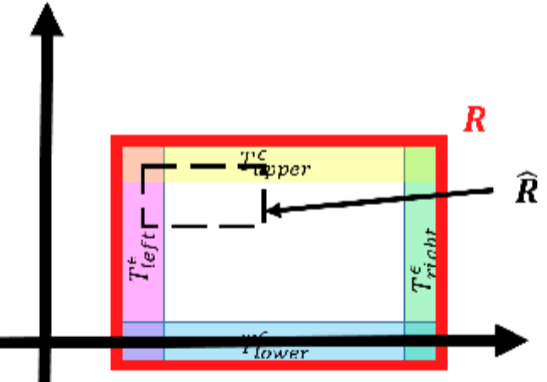
\includegraphics[width=\columnwidth]{images/13-rig}
	\end{center}
\end{minipage}

\subsubsection*{2. Prove $\P(\mathcal R(\hat R)\leq \epsilon) \geq \P(\RIG)\geq 1 - 4\exp\left(-\frac{n\epsilon}{4}\right)$}
\begin{itemize}
	\item Learning algorithm: "tightest fitting rectangle"
	\item Determine
	\begin{align*}
		x_1^{min} = \min\{x_{1,c}:1\leq i\leq n\} \\
		x_1^{max} = \max\{x_{1,c}:1\leq i\leq n\} \\
		x_2^{min} = \min\{x_{2,c}:1\leq i\leq n\} \\
		x_2^{max} = \max\{x_{2,c}:1\leq i\leq n\} \\
	\end{align*}
	\item Select Rectangle $\hat R = \square(x_1^{min}, x_1^{max}, x_2^{min}, x_2^{max})$
\end{itemize}

\textbf{Error: }
\begin{align*}
	\P(\textit{"error"}) 	&= \P(R\Delta\hat R) \\
							&= \P(R - \hat R)\cup (\hat R - R) = \P(R - \hat R)\\
	P(R - \hat R) 			&= \P(\textit{top strip} \cup \textit{bottom s.} \cup \textit{left s.} \cup \textit{right s.}) \\
							&\leq \P(\textit{top}) + \P(\textit{bottom}) + \P(\textit{left}) + \P(\textit{right}) 
\end{align*}

Since the probability to be in one of the strips is $\frac{\epsilon}{4}$ for each strip, we get:
\begin{align*}
	\P(\textit{no sample in top strip)} &= \left(1-\frac{\epsilon}{4}\right)^n \\
	\P(\textit{no sample in any strip)} &\leq 4\left(1-\frac{\epsilon}{4}\right)^n \\
										&\leq 4\exp\left(\frac{n\epsilon}{4} \right)
										&\leq \delta
\end{align*}

Rectangles are PAX learnable, since $n'\geq \frac{4}{\epsilon}\geq \frac{4}{\epsilon}\log\frac{4}{\epsilon}$: 

\begin{align*}
		\P(R\Delta \hat R < \epsilon) &\geq 1 - 4\exp\left(\frac{n\epsilon}{4} \right) \\
		\P(R\Delta \hat R \geq \epsilon) &\leq \underbrace{4}_{\textit{Complexity}}\underbrace{\exp\left(\frac{n\epsilon}{4} \right)}_{\textit{model fit.}} \\
\end{align*}

\subsubsection{Error Prob. for realizable finite hypothesis classes $\mathcal H = \mathcal C$}

$\mathcal C$ finite, $\mathcal H = \mathcal C$, consistent hypothesis $\hat c$ $\forall n< \infty: \hat{\mathcal R}_n(\hat c) = 0$ for any target concept $c\in \mathcal C$, $\hat c\in\argmin_{c\in\mathcal C} \hat R_n(c)$

\begin{align*}
	\P(R(\hat c > \epsilon) &= \P(\max_{c\in\mathcal X:\hat R_n=0} R(x) > \epsilon) \\
							&\leq \sum_{c\in\mathcal C} \P(R(c) > \epsilon\land \hat R_n(c) = 0) \\
							&\leq |\mathcal C|(1-R(c))^n \leq |\mathcal C|e^{n\epsilon} \leq \delta \\
							&\leq |\mathcal C|(1-\epsilon)^n \leq |\mathcal C|e^{n\epsilon} \leq \delta \\
	\implies -n\epsilon + \log|\mathcal C| &\leq \log\delta \\
	\implies n&\geq \frac{1}{\epsilon}\left(\log|\mathcal H| + \log\frac{1}{\delta} \right)
\end{align*}

Further: 
\begin{align*}
	\P(\mathcal R(\hat c)\leq \epsilon) &\geq 1 - \delta &\textit{ bounds the success probability $\delta$}\\
	\P(\mathcal R(\hat c)> \epsilon) &\leq \delta 		&\textit{ bounds the error probability $\epsilon$}
\end{align*}

\begin{highlight}{Proving (efficient) PAC learnability}
\textit{To prove PAC learnability, we have to show that}
$$
	\P(\mathcal R(\hat{c}_n^*) \leq \epsilon) \geq 1 -\delta
$$
\textbf{Efficient PAC learnability: }\\ 
Show the algorithm runs polynomial in $\frac{1}{\delta}$ and $\frac{1}{\epsilon}$
\sepline
\textbf{Example in Exercise 8.3 (Concentric Circles).}
\end{highlight}

\subsubsection{The general stochastic setting}
In general, an instance's label is not determined by the underlying concepts. We model this by distribution $\mathcal D$ on $\mathcal X\times \{0,1\}$. (e.g. two patients with similar features have different reactions on same drug).

\begin{itemize}
	\item Training dataset: $\mathcal Z=\{(x_1, y_1), ..., (x_n, y_n)\}$ from $\mathcal D$.
	\item Goal: Find hypothesis $\hat c\in \mathcal H$ with small generalization error 
	$$
		\mathcal R(\hat c) = \P_{x,y\sim \mathcal D}(\hat c(x)\neq y) = \E_{x,y\sim \mathcal D}\left(\mathbf 1_{\hat c(x)\neq y}\right)
	$$
	\item If the bayes optimimal classifier is not in the hypothesis class $\mathcal C$, then it is \textbf{impossible to attain} $\forall 0 < \epsilon \leq \frac{1}{2}:\mathcal R(\hat c)\leq \epsilon$. Instead, we aim to attain the best solution given in the hypothesis class:
	$$
		R(\hat c) - \inf_{c\in\mathcal C}\mathcal R(c) \leq \epsilon
	$$
\end{itemize}

\subsubsection{The general PAC model}
A learning algorithm $\mathcal A$ can learn a concept class $\mathcal C$ from $\mathcal H$ if given {\color{imp3}sufficiently large sample} as input, outputs a hypothesis that \textbf{{\color{imp}generalizes well} {\color{imp2}with high probability}}

\textbf{Definition: } A learning algorithm $\mathcal A$ can learn a concept class $\mathcal C$ from $\mathcal H$ if there is a {\color{imp3} polynomial function $\mathit{poly}$}, such that
\begin{enumerate}
	\item For any distribution $\mathcal D$ on $\mathcal X\times \{0,1\}$ and
	\item for any {\color{imp}$0<\epsilon<1/2$} and {\color{imp2}$0<\delta<1/2$}
\end{enumerate}
if $\mathcal A$ receives as input {\color{imp3} a sample $\mathcal Z$ of size $n\geq \mathit{poly}(1/\epsilon, 1/\delta, \mathit{dim}(\mathcal X)$}, then $\mathcal A$ outputs $\hat c\in\mathcal H$, sucht that
$$
	{\color{imp2}\P_{\mathcal Z\sim \mathcal D^n}\left({\color{imp}\mathcal R(\hat c) - \inf_{c\in\mathcal C}\mathcal R(c)\leq \epsilon }\right) \geq 1 - \delta}
$$

\begin{highlight}{Proving PAC learnability in the General stoch. setting}
\textit{To prove PAC learnability, we have to show that}
$$
	\P(\mathcal R(\hat{c}_n^*) - \inf_{c\in \mathcal C} \mathcal R(c) \leq \epsilon) \geq 1 - \delta
$$

\sepline
\textbf{Example (ex. 8.2): }
Given: \\
$\P(\mathcal R(\hat{c}_n^*) - \inf_{c\in \mathcal C} \mathcal R(c) > \epsilon) \leq \exp(-\epsilon n)$

\begin{enumerate}
	\item Set $\P(\mathcal R(\hat{c}_n^*) - \inf_{c\in \mathcal C} \mathcal R(c) > \epsilon) \leq \exp(-\epsilon n) {\color{imp}\leq \delta}$
	\item Find $n$ sucht that $\exp(-\epsilon n) \leq \delta$
	\item Observe that for this $n$
	\begin{equation*}
		\begin{gathered}
			1 - \P(\mathcal R(\hat{c}_n^*) - \inf_{c\in \mathcal C} \mathcal R(c) \leq \epsilon) \leq \delta \\
			\P(\mathcal R(\hat{c}_n^*) - \inf_{c\in \mathcal C} \mathcal R(c) \leq \epsilon) \leq 1 -\delta
		\end{gathered}
	\end{equation*}
	\textbf{Hence $\mathcal C$ is PAC learnable from itself.}
\end{enumerate}

\end{highlight}

	\section{Computational Learning Theory}
\textbf{Attention: There are different notiations used due to different notations in lecture notes and slides.}

\textit{Minimizing risk is generally unreasonable, because estimating density is more difficult than minimizing the expected risk. It is only plausible if substantial prior information on $\P(x,y)$ is available and $\P(x,y)$ can be defined up to its parameters. (Vapnik, 1982)}
\subsection{Empirical Risk Minimization}
\begin{itemize}
	\item Induction principle: Empirical Risk Minimization. Select the classifier $\hat c_n^*\in\mathcal C$ with the smallest error on the training data $\mathcal Z=\{(x_1, y_1), ... (x_n, y_n)\}$
	$$
		\hat c_n^* = \argmin_{c\in\mathcal C}\underbrace{\frac{1}{n}\#\{(x_i, y_i):c(x_j)\neq y_j, 1\leq i\leq n\}}_{\textit{Training error $\hat{\mathcal R}_n(c)$}}
	$$
	\item Empirical Classification Error: $\hat{\mathcal R}_n(c) = \frac{1}{n}\sumj n \mathbb I_{\{c(x_j)\neq y_j\}}$
	\item Expected Classification Error $\mathcal R(c) = \P\{c(X)\neq Y\}$ is the quality measure which we care about.
	\item \textbf{Goal: } Derive a distribution independent bound for the prob. of larve deviatons between the expected risk of the ERM classifier and the opimal classifier:\\
		$\P\{\mathcal R(c_n^*)-\inf_{c\mathcal C}\mathcal R(c) > \epsilon\}$
	 \item Generalization Error: $\mathcal R(c_n^*)=\P\{c_n^*(X)\neq Y|\mathcal Z\}$
	 \item \textbf{Problem: } we cannot measure $\mathcal R(c_n^*)$
\end{itemize}

\subsection{VC inequality}
\textbf{How can we bound the difference between expected risk $R(x)$ and empirical risk $\hat R_n(x)$?} Vapnik-Chervonenkis Inequality.

\begin{itemize}
	\item $\hat c \in \argmin_{c\in\mathcal C} \hat R_n(c) = \argmin_{c\in\mathcal C} |\{\hat c(x_i)\neq y_i\}|$ \\is the minimizer of emirical risk and
	\item $c^*\argmin_{c\in\mathcal C} R(c)$ is the minimizer of the expected risk.
\end{itemize}

Consider
\begin{align*}
	R(\hat c) - \inf_{c\in\mathcal C}R(c) 	&= \underbrace{R(\hat c) - \hat R_n(\hat c)}_{\leq\sup_{c\in\mathcal C}|R(c) - \hat R_n(c)|} + \underbrace{\hat R_n(\hat c)}_{\leq \hat R_n(c^*)} - R(c^*) \\
											&\leq \sup_{c\in\mathcal C}|R(c) - \hat R_n(c)| 
												+ \underbrace{\hat R_n(c^*) - R(c^*)}_{\leq\sup_{c\in\mathcal C} |R(c) - \hat R_n(c)|}\\
											&\leq 2 \sup_{c\in\mathcal C}|R(c) - \hat R_n(c)| 
\end{align*}
The difference between the expected risk of the ERM and smallest expected risk is bounded by twice the worst derivation of expected from empirical risk!

\subsubsection{Error Probability Bounds: }
\begin{align*}
	\P(R(\hat c) - \inf_{c\in\mathcal C}R(c) \geq\epsilon) 	&\\
	\textit{(VC Inequality)}									&\leq \P(\sup_{c\in\mathcal C}|R(c) - \hat R_n(c)|) \\
	\textit{(Union Bound)}									&\leq \sum_{c\in\mathcal C}\P\left(|R(c) - \hat R_n(c)|\geq\frac{\epsilon}{2}\right) \\
															&= \mathit{ub}(n, \epsilon) = \delta
\end{align*}
(\textit{Union Bound: $\P(e_1\lor e_2 \lor ... \lor e_k)\leq \sum P(e_j)$})

Solving the last equation we get: 
\begin{align*}
	\mathit{ub}(n, \epsilon) 	&= \delta \\
		\implies	\epsilon		&= \mathit{st}(n, \delta) 
\end{align*}

We have $|R(c) - \hat R_n(c)| <\frac{\epsilon}{e} = \mathit{st}(n, \delta)$ with high probability $1-\delta$

We can bound an expected cost by
$$
	\forall c\in\mathcal C: R(c) < \underbrace{\hat R_n(c)}_{\textit{computable}} + \underbrace{\frac{1}{2} \mathit{st}(n,\delta)}_{\textit{overfitting correction}}
$$

\textit{Risk bounding is a difficult task. In classification, the risk is bounded by $0\leq R(c)\leq 1$. Therefore we can achieve distribution independent bounds.}


\subsubsection{Strategies for tight(er) bounds:}
\begin{itemize}
	\item Estimate how different are functions when they are evaluated on finite samples
	\item Approximate unknown true distribution by empirical distribution
\end{itemize}

\subsubsection{Hoeffding's Inequality}
(I think this was not in the lecture)

{\color{gray}
\textbf{Lemma 2: } (\textit{Markov inequality) Let X be a non-negative random variable. Then}
$$
	\P\{X\geq \epsilon\}\leq \frac{\E[X]}{\epsilon}
$$

\textbf{Lemma 3} \textit{Let $X$ be a random variable with $\E[X]=0$ and $a\leq X\leq b$. Then for $s>0$ it holds that}
$$
	\E[\exp(sX)]\leq \exp(s^2(b-a)^2/8)
$$

\textbf{Hoeffding's Theorem / Chernoff Bound} \textit{Let $X_1, ..., X_n$ be independent bounded random variables such that $X_i$ falls in the interval $[a_i, b_i]$ with probability 1 and let $S_n=\sumi n X_i$. Then for any $t>0$ we have }
\begin{align*}
	\P\{S_n - \E [S_n]\geq t\} & \leq \exp\left(-\frac{2t^2}{\sumi n (b_i - a_i)^2} \right) \\
	\P\{S_n - \E [S_n]\leq -t\} & \leq \exp\left(-\frac{2t^2}{\sumi n (b_i - a_i)^2} \right)
\end{align*}
}

\end{multicols*}

\end{document}